% Chapter 4
%----------------------------------------------------------------------------------------
\chapter{Propuesta de solución} % Main chapter title
\label{Chapter4} % For referencing the chapter elsewhere, use \ref{Chapter4} 
\begin{onehalfspacing}

\section{Metodología}
\label{sec:Metodologia}

La metodología que se presenta se basa en la hipótesis propuesta y en la Figura \ref{fig:Fig_Metodologia}, se muestra un esquema de la metodología que se utilizará para probar la hipótesis y a continuación una sección explicando cada uno de los pasos.

\begin{figure}[h!]
	\centering
	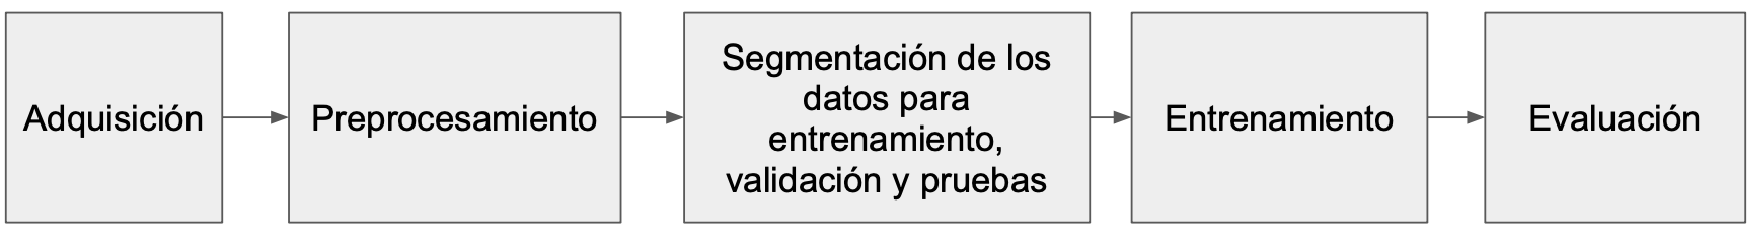
\includegraphics[width=18cm,keepaspectratio]{XX_Figures/Fig_Metodologia.pdf}
	\caption{\footnotesize Metodología propuesta para detectar mentiras en videos.}
	\label{fig:Fig_Metodologia}
\end{figure}

\subsection{Adquisición}
\label{sec:Adquisicion}
Al inicio se debe descargar o crear un conjunto de datos en la cuál se podrán hacer las pruebas de las hipótesis propuesta; este conjunto de datos debe contener videos con resoluciones medias tales cómo 480p o 720p(HD). Los formatos de los videos en WMV, MP4, MOV, AVI o FLV, con los 3 planos RGB. En los videos deben aparecer personas con declaraciones falsas y verdaderas. Estas personas también deben aparecer en todos los fragmentos del video para evitar el análisis de otros factores que no tengan que ver con el movimiento y la silueta del individuo. Nos podemos referir como \textit{frames} a los fotogramas que tiene un video ya que en varios trabajos en inglés y español es utilizado.\\

\subsection{Preprocesamiento}
\label{sec:Preprocesamiento}
Para el preprocesamiento de los videos se ocuparán librerías de OpenCV en python las cuáles han sido ocupadas para diferentes tareas que requieren de visión artificial, tales como reconocimiento de objetos, detección de movimientos, obtención de filtros espaciales, redimensionamiento, agudización de los frames, entre otros. A continuación se listan los pasos a seguir en el preprocesamiento:


\begin{enumerate}
    \item Obtener la separación de cada uno de los canales R,G,B Y la escala de grises promediada de cada uno de los fotogramas en los videos. La Figura \ref{fig:Fig_Dataset1_RGB_GS} muestra este procedimiento y la explicación de los canales RGB se encuentran la sección del Marco Teórico \ref{RGB} y para la obtención de la escala de grises en la sección del Marco Teórico \ref{GS}.
    \begin{figure}[h!]
    	\centering
    	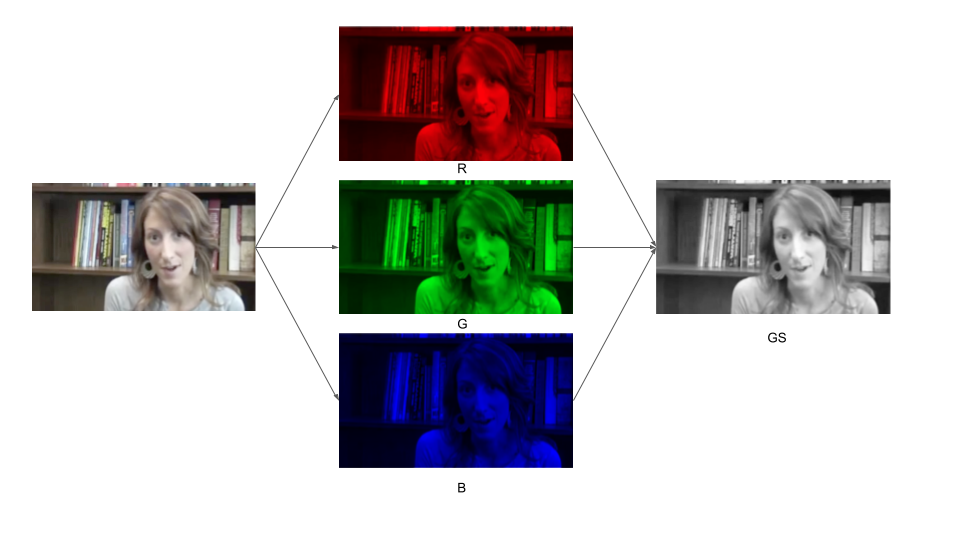
\includegraphics[width=10cm,keepaspectratio]{XX_Figures/Fig_Dataset1_RGB_GS.png}
    	\caption{\footnotesize Separación RGB y escala de grises.}
    	\label{fig:Fig_Dataset1_RGB_GS}
    \end{figure}
    
    \item Recortar los canales RGB de cada fotograma de los videos y la escala de grises (GS) obtenida para evitar tener información que no esté relacionada con el individuo a prueba. La primera propuesta de este recorte es quitando 60 píxeles en la parte superior, 70 en la parte inferior, 70 por la izquierda y 50 por la derecha. Al hacer este procedimiento se obtiene un fotograma como se muestra en la Figura \ref{fig:Fig_Dataset1_Recorte}. La segunda propuesta es recortar la imagen para obtener solamente el rostro del individuo; para lograr esto se utilizaron clasificadores en cascada basados en funciones de Haar, el cuál a través de aprendizaje profundo, la función de cascada se entrena a través de gran cantidad de imágenes positivas (imágenes con caras) y negativas (imágenes sin caras) para luego ser utilizada en detección de rostros en otras imágenes.  
    \begin{figure}[h!]
    	\centering
    	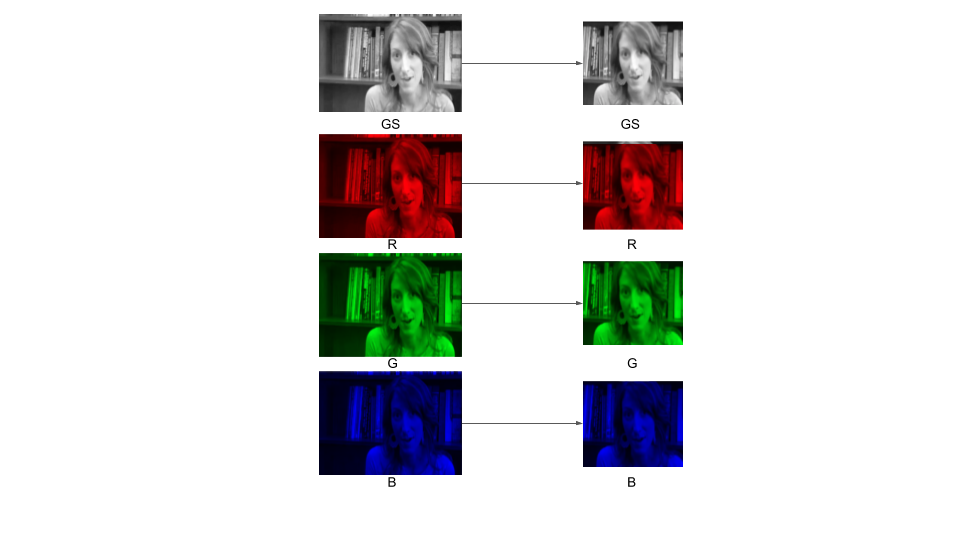
\includegraphics[width=12cm,keepaspectratio]{XX_Figures/Fig_Dataset1_Recorte.png}
    	\caption{\footnotesize Recorte de los fotogramas.}
    	\label{fig:Fig_Dataset1_Recorte}
    \end{figure}

    \item Aplicar redimensión a R,G,B y GS para reducir el tamaño de los datos con el costo de perder calidad de información pero reduciendo el costo computacional de las operaciones que se realizarán a cada uno de los fotogramas. Para el redimensionamiento se ocupará la función \textit{resize} de la librería de OpenCV, con interpolación \textit{InterArea} la cuál obtiene el promedio de gran cantidad de píxeles. Esta interpolación es muy útil para achicar una imagen pero mala para agrandarla. Al final de este procedimiento se obtiene una imagen de (y,x) píxeles. En la Figura \ref{fig:Fig_Dataset1_Redimensionar} se muestra un ejemplo de un fotograma extraído de un video en HD para obtener un fotograma con tamaño 100 x 100.
    \begin{figure}[h!]
    	\centering
    	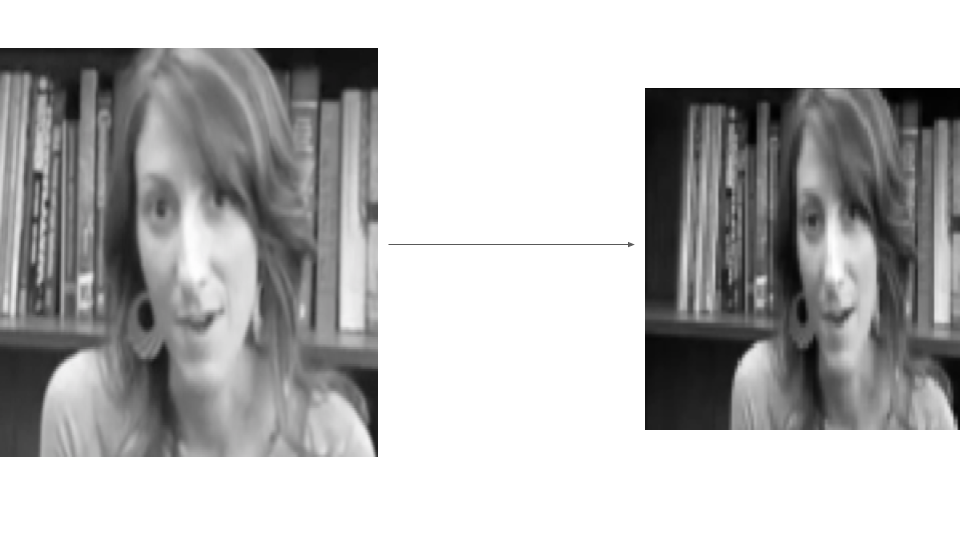
\includegraphics[width=12cm,keepaspectratio]{XX_Figures/Fig_Dataset1_Redimensionar.png}
    	\caption{\footnotesize Redimensionamiento de los fotogramas de un video HD (1280x720) a 100x100 pixeles.}
    	\label{fig:Fig_Dataset1_Redimensionar}
    \end{figure}

    \item Aplicar los filtros SobelX (SX), SobelY(SY) y Kirsh (K) para obtener las siluetas y bordes de los objetos, OpticalFlowX(OX) y OpticalFlowY(OY) para obtener el movimiento de un fotograma con respecto a otro consecutivo y Laplaciano (L) para agudizar los fotogramas. Cada uno de estos filtros son explicados en la sección \ref{Filtros_espaciales} del Marco Teórico. En la Figura \ref{fig:Fig_Dataset1_Filtros} se muestra un ejemplo de la obtención de estos filtros con el filtro escala de grises (GS).
    \begin{figure}[h!]
    	\centering
    	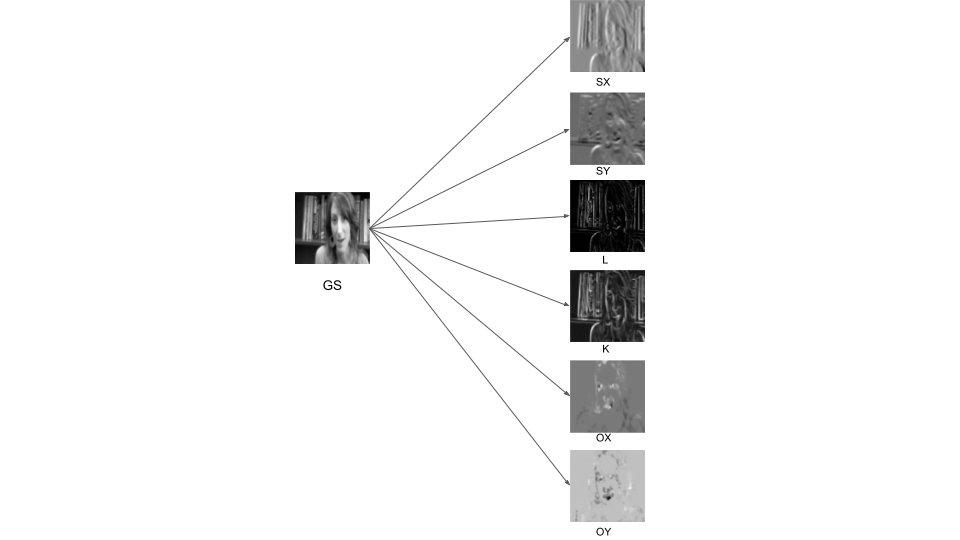
\includegraphics[width=18cm,keepaspectratio]{XX_Figures/Fig_Dataset1_Filtros.png}
    	\caption{\footnotesize Obtención de los canales SX,SY,OX,OY,L y K.}
    	\label{fig:Fig_Dataset1_Filtros}
    \end{figure}
    
    \item División de los videos en fragmentos: Cada uno de los videos se fragmentará en n número de fotogramas, ya que se desea probar si con pequeños fragmentos de videos con n número de fotogramas es suficiente para reconocer mentira o verdad en una persona. Los formatos y la cantidad de fotogramas por segundo que tiene un video pueden cambiar, por ejemplo si se tiene un video a 30 FPS (60 Hz), se puede convertir a 15 FPS si se toman la mitad de los fotogramas del video a 30 FPS pero con la misma cantidad de tiempo; esto se puede lograr tomando como separación un fotograma entre cada fotograma que se ocupe. A este procedimiento lo llamaremos \textbf{FrameSpace} y se refiere a la cantidad de espacios (fotogramas) que hay entre los fotogramas seleccionados, este procedimiento se puede apreciar en la Figura \ref{fig:Fig_FrameSpace} y se utilizará para saber a que velocidad de fotogramas se pueden detectar mentiras y verdades. Al final de este proceso se obtendrá lo que llamaremos un \textbf{dato}, el cual consiste en n cantidad de fotogramas, con c cantidad de canales y dimensión espacial (y,x). En la Figura \ref{fig:Fig_Dato7Frames}, se observa un ejemplo de un dato x que contiene n = 7 fotogramas, c = 3 canales (RGB), (y,x) = 100x100 píxeles. Schindler \cite{SchindlerVanRequire} menciona que de 1 a 7 fotogramas a 25 Hz (25 Hz $\simeq$ 13 FPS) es suficiente para reconocer acciones humanas y en \cite{Ji20133DRecognition} solamente necesitaron de 7 fotogramas para detectar acciones humanas con una mayor precisión que tomando todo los fotogramas de un video, esto motivó a que el modelo piloto tuviera como entrada datos de 7 fotogramas y los canales RGB.
    
    \begin{figure}[h!]
    	\centering
    	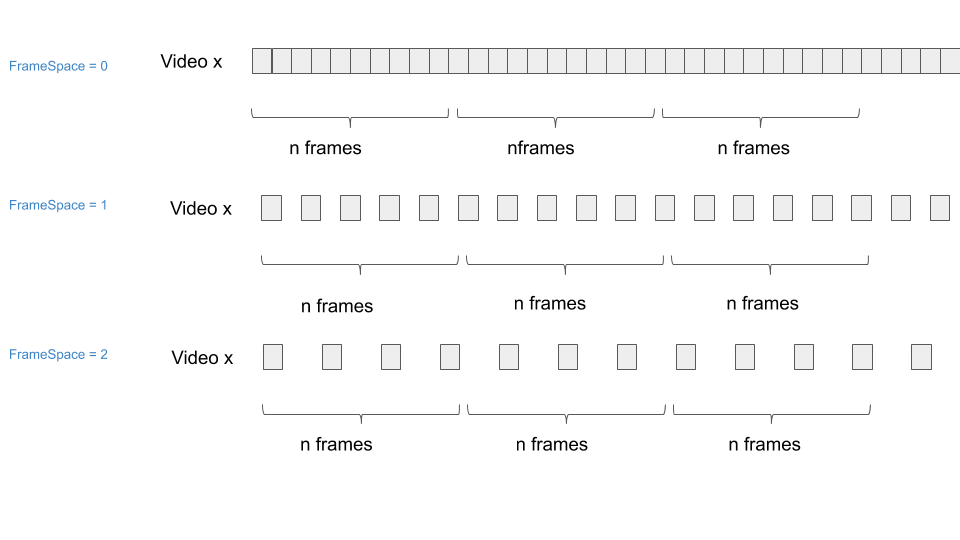
\includegraphics[width=14cm,keepaspectratio]{XX_Figures/Fig_FrameSpace.png}
    	\caption{\footnotesize Funcionamiento de FrameSpace.}
    	\label{fig:Fig_FrameSpace}
    \end{figure}
    
    \begin{figure}[h!]
    	\centering
    	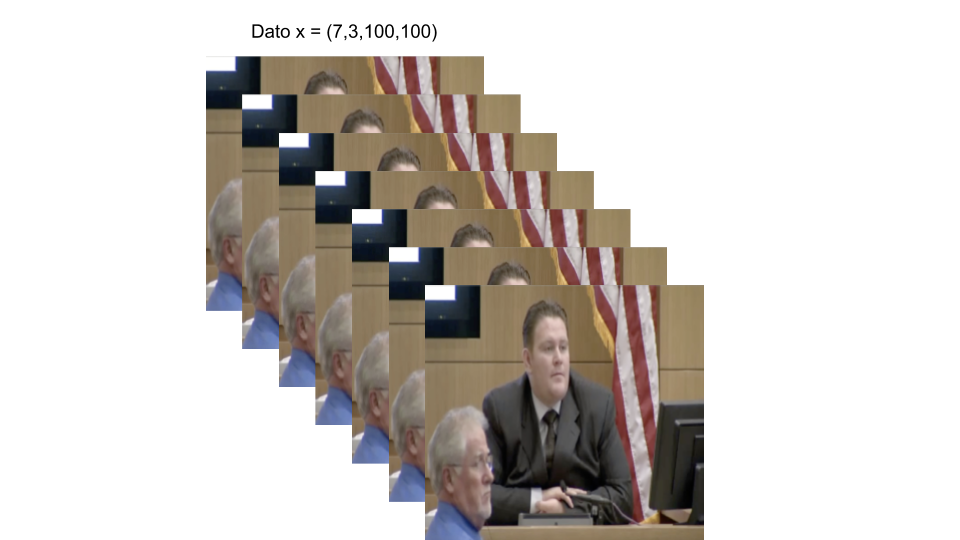
\includegraphics[width=12cm,keepaspectratio]{XX_Figures/Fig_Dato7Frames.png}
    	\caption{\footnotesize Ejemplo de un dato.}
    	\label{fig:Fig_Dato7Frames}
    \end{figure}
    
    \item Cada uno de los datos se etiquetan con [1,0] en el caso de pertenecer a un video de mentira o [0,1] en el caso de pertenecer a un video de verdad. En la Figura \ref{fig:Fig_Etiqueta_datos} se muestra un ejemplo en la que \textit{m} datos pertenecientes a un video de mentira son etiquetados con [1,0] indicando que son datos de mentira y \textit{v} datos pertenecientes a un video de verdad son etiquetados con [0,1] indicando que son datos de verdad.
\end{enumerate}

\begin{figure}[h!]
    	\centering
    	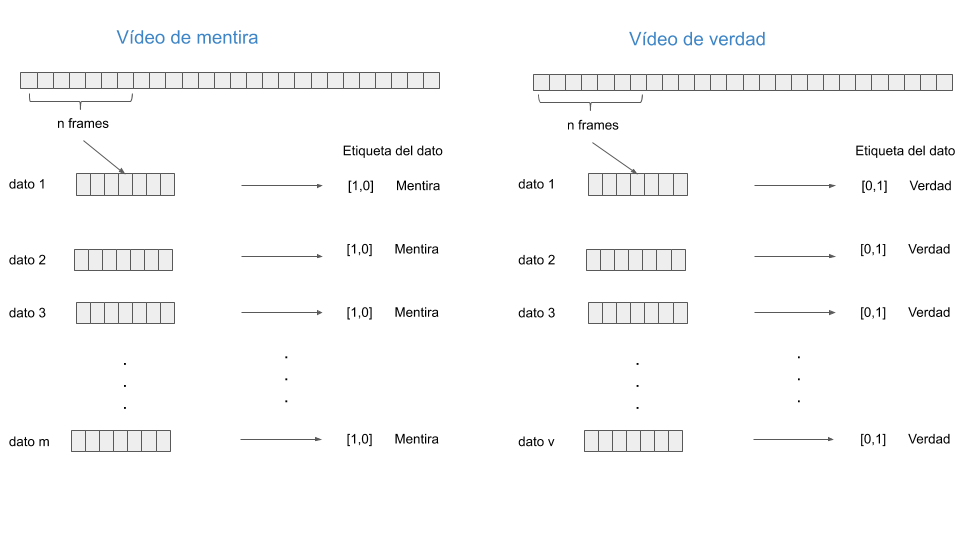
\includegraphics[width=17cm,keepaspectratio]{XX_Figures/Fig_Etiqueta_datos.png}
    	\caption{\footnotesize Etiquetado de los datos.}
    	\label{fig:Fig_Etiqueta_datos}
\end{figure}

%---------------------------------------------
\subsection{Segmentación de los datos}
\label{sec:Segmentacion datos}
Los datos se segmentarán de la siguiente manera: 
\begin{itemize}
    \item  El primero conjunto de datos es el Train en el cuál están la mayoría de los datos; esto es para que se la red tenga suficientes datos que le permitan generalizar o al menos conocer las suficientes situaciones en las que necesite clasificar nuestro problema. Estos datos de entrenamiento contienen \textit{D} datos etiquetados como mentira y \textit{T} datos etiquetados como verdad los cuales serán barajeados (shuffle) aleatoriamente. Una vez combinados los \textit{n} datos de entrenamiento, se dividirán en lotes (batches) con \textit{m} cantidad de datos. Cada uno de los batches pasarán por las etapas de entrenamiento explicadas posteriormente en la subsección \ref{sec:Entrenamiento} y al terminar de pasar todos los batches, habrá terminado la primera época de entrenamiento. Este procedimiento se repite \textit{e} cantidad de veces, dependiendo del número de épocas. Entre más grande sea el tamaño del batch, más capacidad computacional será necesaria para entrenar los datos.
    \item El segundo conjunto es el Validation en la cuál se extrae un pequeño conjunto de datos del Train para notar como se comporta la red con datos muy parecidos pero nunca antes vistos. Este conjunto se evalúa al terminar una época de entrenamiento.
    \item El último conjunto es el Test en la cuál se harán las pruebas para conocer la robustez y la confiabilidad del sistema; aquí por lo general los datos son diferentes que el conjunto de Train y Validation. Este conjunto se evalúa después de e épocas propuestas.
\end{itemize}

\subsection{Entrenamiento}
\label{sec:Entrenamiento}

\subsubsection{Entradas y salidas}
\label{sec:Entrada}

Para la entrada al modelo los datos consistirán en \textit{d = (f,c,y,x)} en dónde \textit{f = número de fotogramas}, \textit{c = número de canales}, y \textit{(y,x)= (altura,ancho)} del fotograma.\\
Debido a que se tiene una codificación \textit{One Hot} en las etiquetas de cada dato como se muestra en la Figura \ref{fig:Fig_Etiqueta_datos}, al final el modelo dará como salida un vector con dos valores, en la cuál el valor más grande representará cómo fue clasificado el dato.

\subsubsection{Arquitectura}
\label{sec:Arquitectura}

Al inicio de la arquitectura, los datos \textit{d = (f,c,y,x)} pasarán por una red convolucional 3D que será la encargada de la extracción de características. Se desea tener un vector \textit{v} a la salida de la red convolucional 3D, por lo tanto dependiendo de dimensiones espaciales en los fotograma \textit{(y,x)}, combinaciones de canales \textit{c} y cantidad de fotogramas \textit{f}, pueden variar la cantidad de capas convolucionales y maxpooling, dando como resultado diferentes arquitecturas. el vector de características \textit{v} se convertirá en la entrada de las capas completamente conectadas en cuál tendrá $C_{mlp}$ capas con diferentes números de neuronas y diferentes funciones de activación. Al final se tendrá una capa de salida con dos neuronas. Con fines visuales, para la arquitectura mostrada a continuación se ocupó como entrada datos de 7 fotogramas con 3 canales (R,G,B) y con dimensiones espaciales de 100x100 píxeles, con el fin de explicar el funcionamiento de la red 3DCNN. Por lo tanto los datos tienen los siguientes valores $${d = (7,3,100,100)}$$ Los pasos se describen a continuación:\\

\begin{enumerate}
    \item Cada uno de los canales se agrupa por separado con sus 7 fotogramas correspondientes, para posteriormente aplicar los filtros convolucionales 3D a cada canal por separado (Figura \ref{fig:Fig_Piloto_p1}).
    
    \begin{figure}[h!]
	\centering
	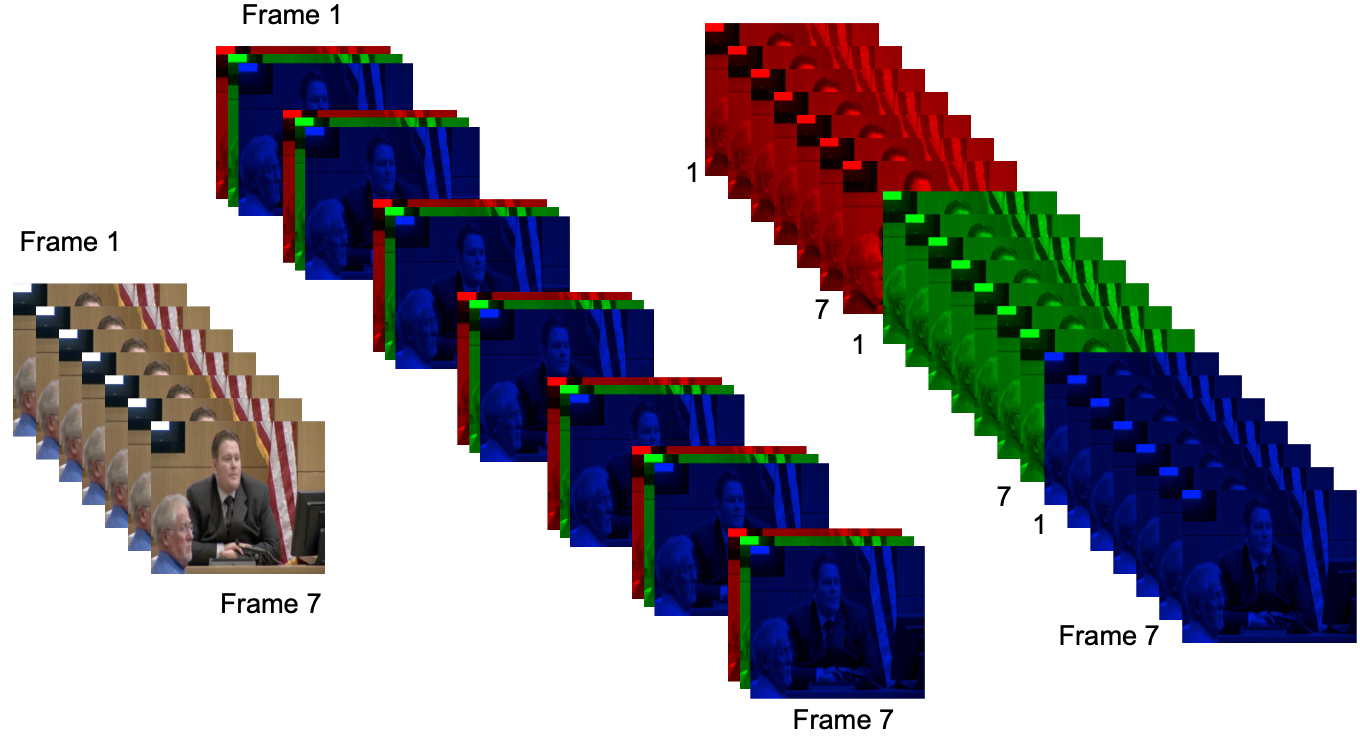
\includegraphics[width=9cm,keepaspectratio]{XX_Figures/Fig_Piloto_p1.png}
	\caption{\footnotesize Separación y agrupación de los canales R,G,B para el modelo piloto.}
	\label{fig:Fig_Piloto_p1}
    \end{figure}
    
    \item Se toma uno de los canales \textit{c} y se le aplicarán \textit {k} kernels convolucionales con dimensión $C = (t_{c},c_{c},x_{c},y_{c})$. Para este ejemplo \textit{k = 4} y cada kernel en esta primera capa convolucional $C1(t,c,y,x) = C1(3,1,3,3)$, tienen un tamaño de $3x3$ en altura y anchura, con una profundidad de canal $c_{c} = 1$(que indica que se aplica la 3DCNN por separado a cada canal) y con dimensión $t_{c}=3$ que indica que se tomarán 3 fotogramas para realizar el paso convolucional. Al aplicar el filtro convolucional 3D con \textit{TemporalStride = 1 y Padding = Same} (sin relleno) se obtienen 4 conjuntos mapas de características, cada uno con 5 matrices y con una anchura y altura de 98x98 respectivamente como se muestra en la Figura \ref{fig:Fig_Piloto_p2}. 
    \begin{figure}[h!]
	\centering
	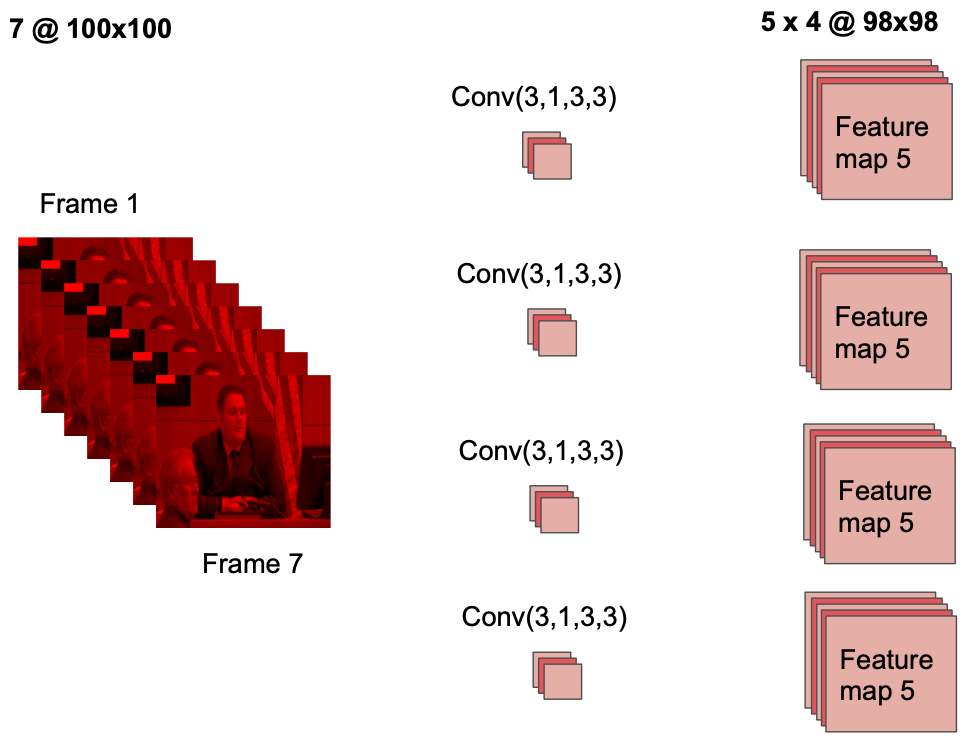
\includegraphics[width=7cm,keepaspectratio]{XX_Figures/Fig_Piloto_p2.png}
	\caption{\footnotesize Aplicación de C1.}
	\label{fig:Fig_Piloto_p2}
    \end{figure}
    
    \item Se aplica un Maxpooling M1 de tamaño \textit{M1(t,y,x) = M1(1,2,2)}, el cual da como resultado los mismos conjuntos de mapas de características pero con una anchura y altura de 49x49 como se muestra en la Figura \ref{fig:Fig_Piloto_M1}.\\
    \begin{figure}[h!]
	\centering
	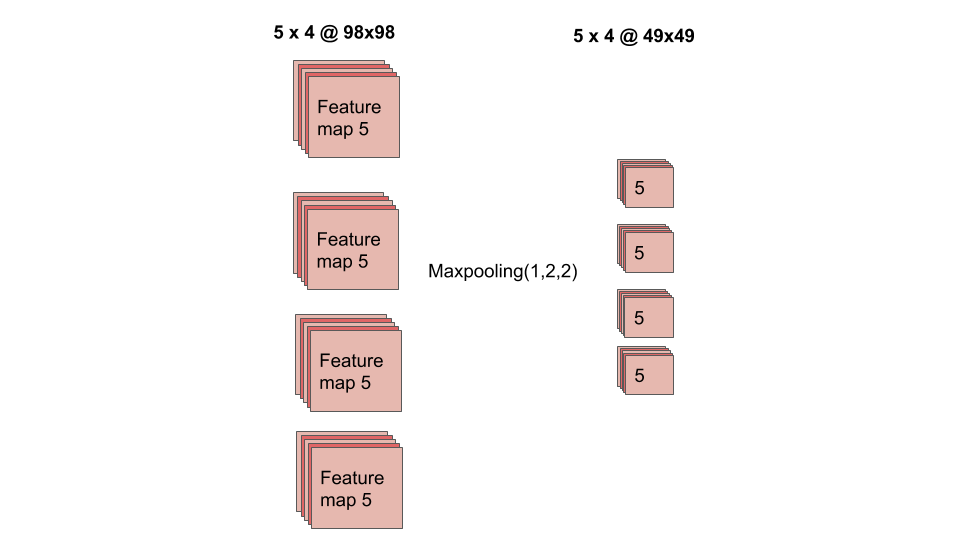
\includegraphics[width=12cm,keepaspectratio]{XX_Figures/Fig_Piloto_M1.png}
	\caption{Aplicación de M1.}
	\label{fig:Fig_Piloto_M1}
    \end{figure}
    
    \item Después se volvieron a aplicar 4 kernels convolucionales 3D pero con valores \textit{C2(3,1,5,5)}, y las mismas características de TemporalStride y Padding. Esto da como resultado 16 conjuntos de mapas de características con 3 matrices cada uno y un tamaño de 45x45 como se muestra en la Figura \ref{fig:Fig_Piloto_C2}.
    \begin{figure}[h!]
	\centering
	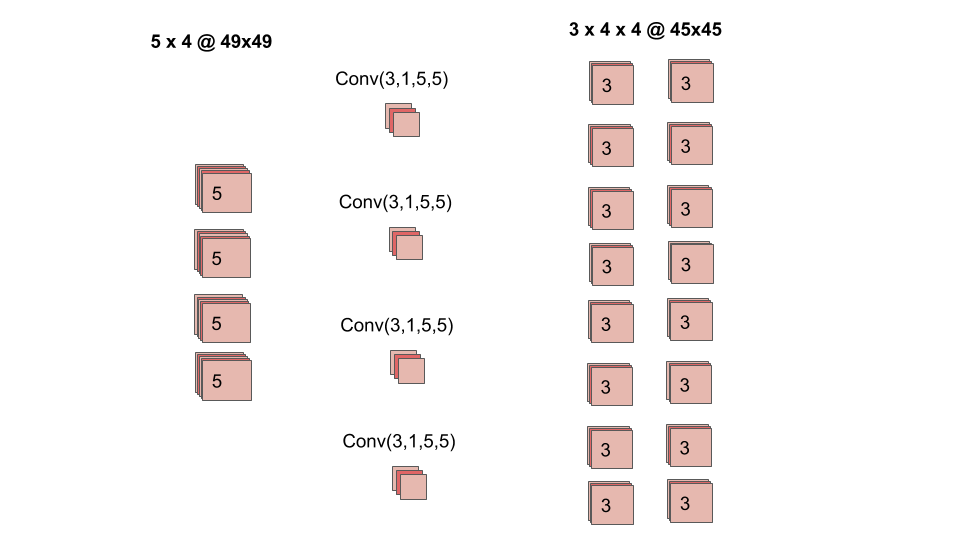
\includegraphics[width=12cm,keepaspectratio]{XX_Figures/Fig_Piloto_C2.png}
	\caption{\footnotesize Aplicación de C2.}
	\label{fig:Fig_Piloto_C2}
    \end{figure}
    
    \item Se aplica un Maxpooling M2 de tamaño \textit{M2(1,5,5)}, el cual da como resultado los mismos conjuntos de mapas de características pero con una anchura y altura de 9x9 respectivamente como se muestra en la Figura \ref{fig:Fig_Piloto_M2}. 
    \begin{figure}[h!]
	\centering
	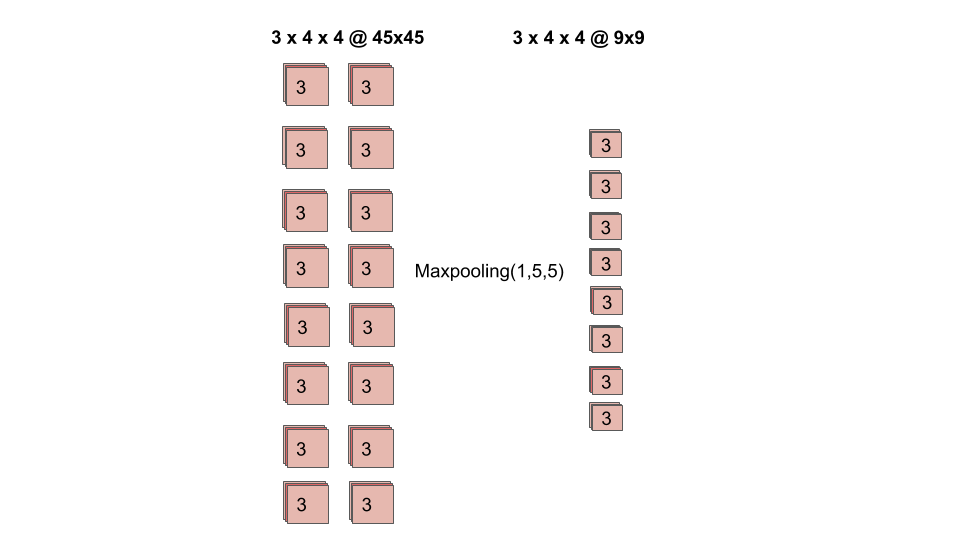
\includegraphics[width=14cm,keepaspectratio]{XX_Figures/Fig_Piloto_M2.png}
	\caption{\footnotesize Aplicación de M2.}
	\label{fig:Fig_Piloto_M2}
    \end{figure}
    
    \item Luego se aplican 2 kernels convolucionales 3D \textit{C3(3,1,5,5)} para obtener 32 conjuntos de mapas de características con 1 matriz por cada conjunto y una dimensión espacial de 5x5 como se muestra en la Figura \ref{fig:Fig_Piloto_C3}.
    \begin{figure}[h!]
	\centering
	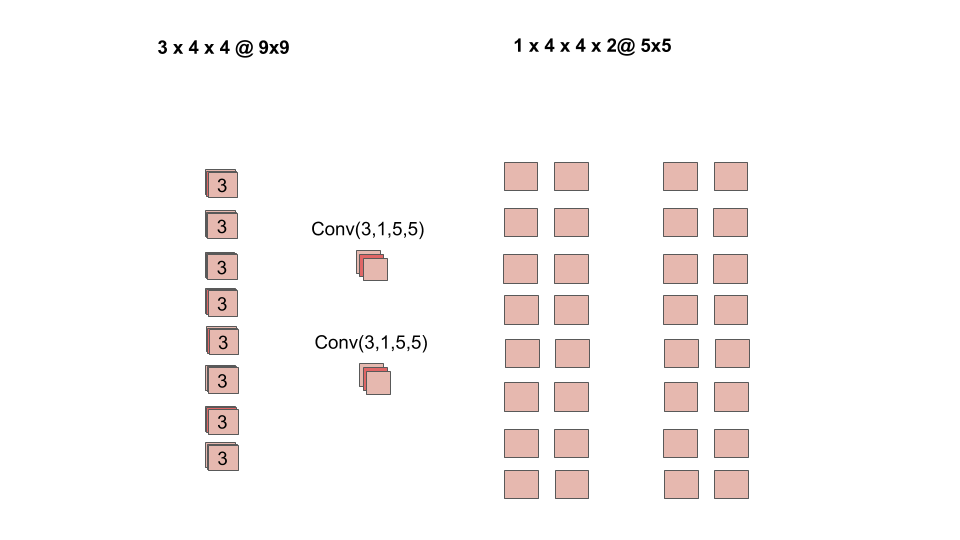
\includegraphics[width=15cm,keepaspectratio]{XX_Figures/Fig_Piloto_C3.png}
	\caption{\footnotesize Aplicación de C3.}
	\label{fig:Fig_Piloto_C3}
    \end{figure}
    
    \item Se aplica un Maxpooling M2 de tamaño \textit{M2(1,5,5)} para obtener un vector con 32 características, las cuales fueron extraídas de un canal con 7 fotogramas (Figura \ref{fig:Fig_Piloto_p5}).
    \begin{figure}[h!]
	\centering
	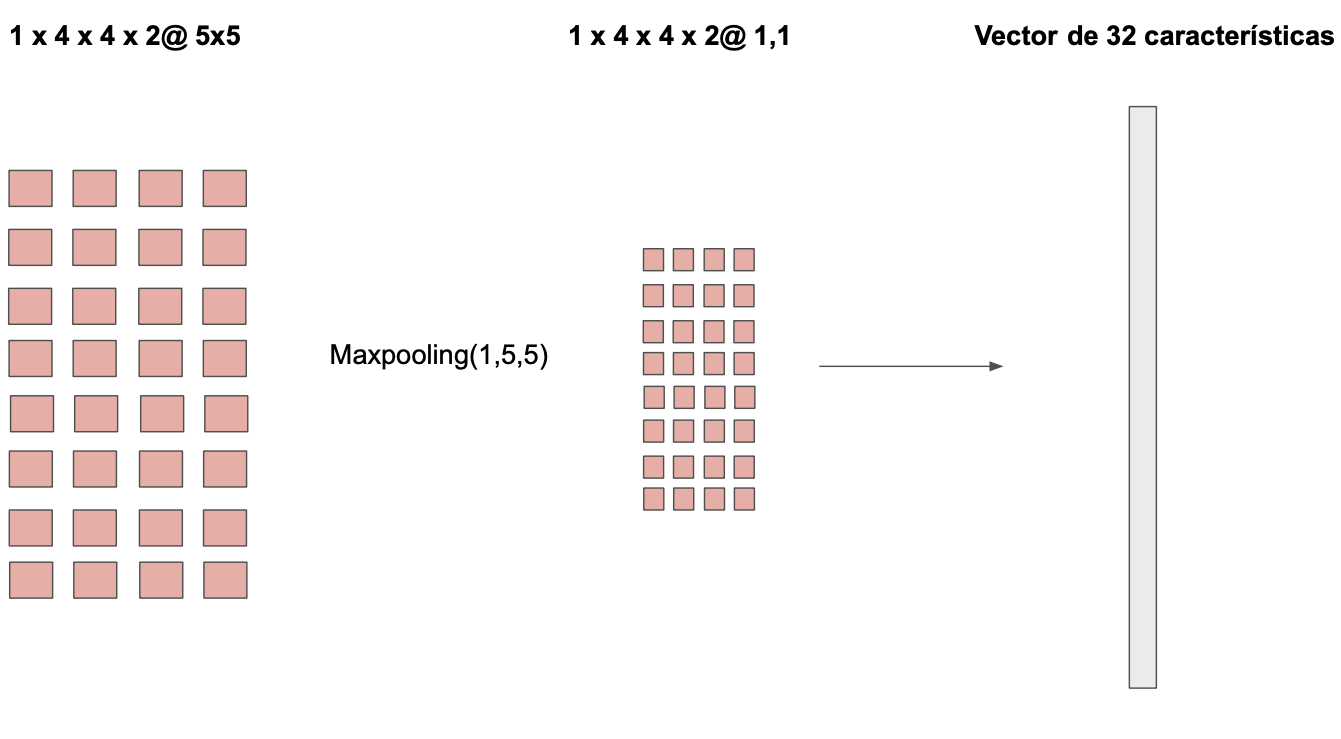
\includegraphics[width=13cm,keepaspectratio]{XX_Figures/Fig_Piloto_p5.png}
	\caption{\footnotesize Aplicación de C5 para obtener vector de características de 32 valores.}
	\label{fig:Fig_Piloto_p5}
    \end{figure}
    
    \item Este mismo procedimiento es aplicado para cada uno de los tres canales y se obtiene un resultado similar como se puede apreciar en la Figura \ref{fig:FIG_3DCNN_DATASET1}, en la cual se muestra al final del proceso los 3 vectores de características obtenidos por los 3 filtros concatenados. Este procedimiento puede ser aplicado para n canales.
    \begin{figure}[h!]
	\centering
	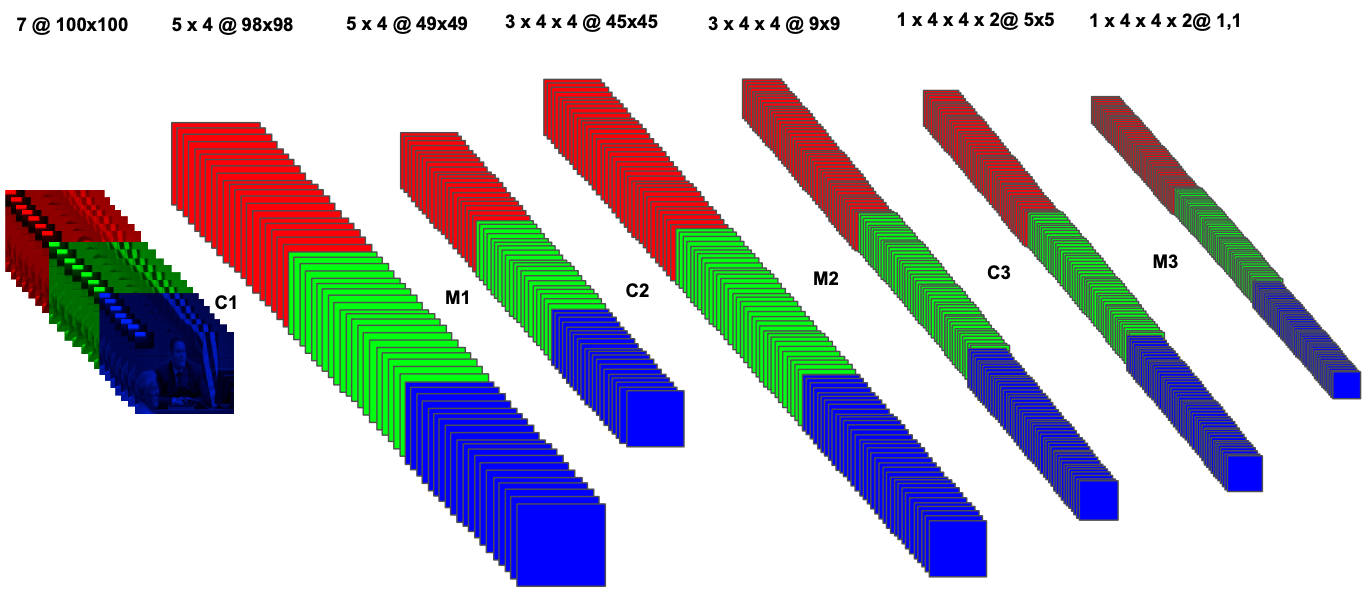
\includegraphics[width=16cm,keepaspectratio]{XX_Figures/FIG_3DCNN_DATASET1.png}
	\caption{\footnotesize Red convolucional 3D.}
	\label{fig:FIG_3DCNN_DATASET1}
    \end{figure}
    
    \item El vector de características concatenado se vuelve la entrada a una MLP profunda con 2 capas ocultas con 96 y 128 neuronas respectivamente y una capa de salida con dos neuronas. Al final se tendrá una clasificación, la cuál será comparada con la etiqueta real. Reduciendo el error obtenido hasta que nuestra condición de paro suceda (Figura \ref{fig:Fig_3DDNN_Piloto}).
    \begin{figure}[h!]
	\centering
	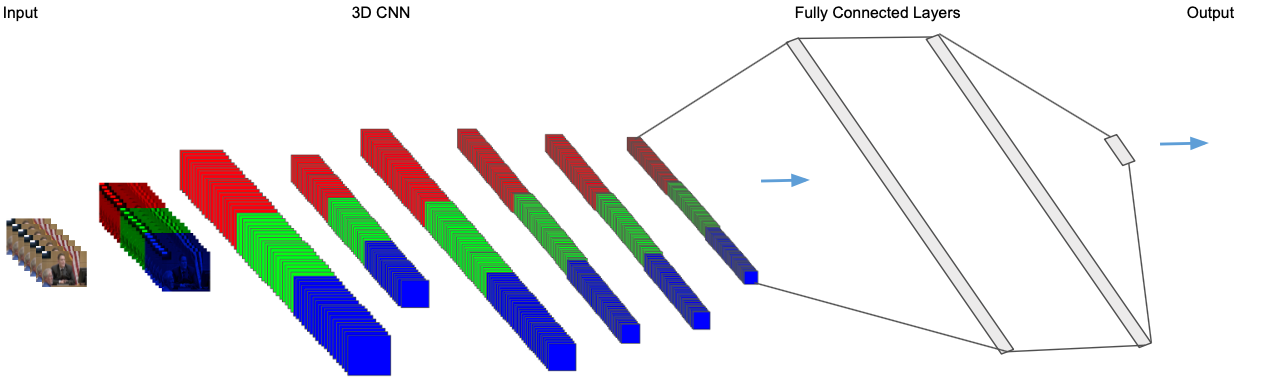
\includegraphics[width=18cm,keepaspectratio]{XX_Figures/Fig_3DDNN_Piloto.png}
	\caption{\footnotesize Arquitectura completa DNN propuesta.}
	\label{fig:Fig_3DDNN_Piloto}
\end{figure}
    
\end{enumerate}


Con este ejemplo se observa que dependiendo de los datos, se pueden construir diferentes modelos con diferentes variedades de filtros convolucionales, capas convolucionales, TemporalStrides, ConvStrides, MaxPoolStrides, etc. De igual forma se pueden construir MLPs con diferentes funciones de transferencia, números de neuronas y de capas ocultas, etc.

\subsubsection{Ajuste de hiperparámetros de entrenamiento}
\label{sec:ajustehiperparametros}
Para calcular el error de salida obtenido por el modelo, se ocupa la función de entropía cruzada (Cross-Entropy). Esta función mide el rendimiento del modelo de clasificación cuyo resultado es un valor de probabilidad entre 0 y 1. La pérdida de entropía cruzada (cross-entropy loss) aumenta a medida que la probabilidad predicha diverge de la etiqueta real y esta es calculada con la ecuación \ref{equ:crossentropy}, donde $p(x)$ es la probabilidad deseada y $q(x)$ es la probabilidad actual. Para disminuir el error obtenido se utilizará el optimizador Adam con valores de Learning rate iniciales entre 0.01 y 0.0001.

\begin{equation}
\label{equ:crossentropy}
    H(p,q) = -\sum_{x}p(x)\log q(x)
\end{equation}



\subsection{Evaluación}
\label{sec:Evaluacion}

Al final de el modelo se debe de evaluar que tan acertado es para detectar mentiras y verdades. La métrica comúnmente utilizada por el estado del arte es la exactitud (accuracy) la cuál es el promedio de los datos clasificados correctamente \cite{Bond2006AccuracyJudgments,Vrij2000DetectingBehavior,Perez-Rosas2015VerbalDetection,KrishnamurthyADetection}. Por ejemplo imaginemos que tenemos 10 datos, 5 son datos con la etiqueta de mentira y 5 con la etiqueta de verdad; El sistema nos arroja que logró clasificar 4 mentiras y 3 verdades correctamente, entonces la exactitud del modelo es de 0.70, convertido a porcentaje es 70\%. Esta exactitud por dato se calcula con la Ecuación \ref{equ:Accuracy}. Se puede referir como \textit{accuracy} a la exactitud.\\

\begin{equation}
\label{equ:Accuracy}
    AccuracyData = \frac{TP+TN}{TP+TN+FP+FN} = \frac{DatosClasificadosCorrectamente}{DatosTotales}
\end{equation}\\


Una propuesta para evaluar el desempeño de los modelos es utilizando una nueva métrica la cuál no evalúa los datos clasificados correctamente, si no que considera los videos que fueron clasificados correctamente. Esta métrica se propuso ya que decidir si una persona mintió o dijo la verdad en todos los fragmentos en los que se segmentó el video podría convertirse en una tarea difícil de clasificar para el modelo.- Para decidir si un video compuesto de n datos es clasificado correctamente se propone que si un video tiene (n/2 + 1) datos clasificados como mentira, entonces hay más probabilidad de que el video pertenezca a esa clase y viceversa.
Al final se obtendrá un accuracy por videos, mostrados por la Ecuación \ref{equ:AccPerVideo}.\\

\begin{equation}
\label{equ:AccPerVideo}
    AccuracyPerVideo = \frac{AccVideo_{0} + AccVideo_{1} + ... + AccVideo_{m}}{m}
\end{equation}\\

donde m es el total de los videos y AccVideo puede tomar 1 si fue clasificado como correcto o como incorrecto.


\section{Datasets}
\label{sec:Datasets}

\subsection{Dataset `Trial'}
\label{sec:Dataset-Trial}

\begin{figure}[th]
	\centering
	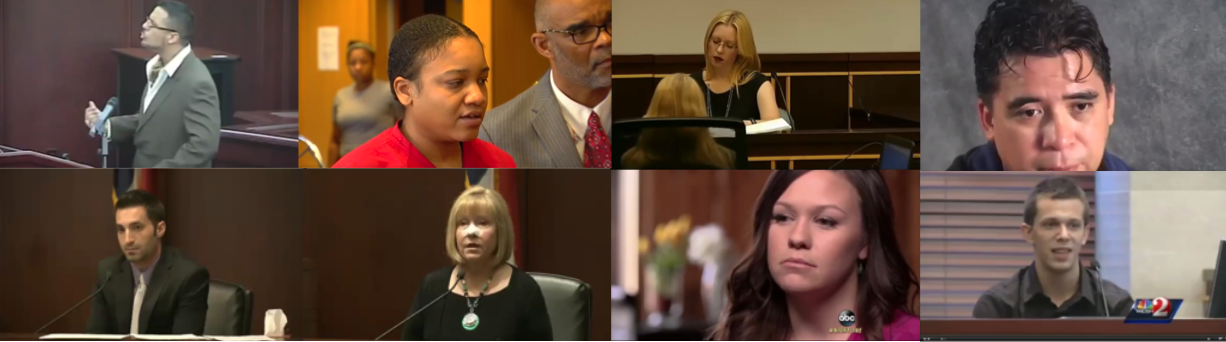
\includegraphics[width=17cm,keepaspectratio]{XX_Figures/Fig_Dataset1.png}
	\caption{\footnotesize Algunos fotogramas de los videos del dataset utilizado en el modelo piloto.}
	\label{fig:Fig_Dataset1}
\end{figure}

El dataset que se propone utilizar ha sido utilizado anteriormente por algunos artículos enfocados a detectar mentiras a través de video \cite{Perez-Rosas2015VerbalDetection,Wu2018DeceptionVideos,KrishnamurthyADetection}. En la Figura \ref{fig:Fig_Dataset1} se observan algunos fotogramas extraídos de 8 videos distintos del dataset `Trial' con diferentes personas, diferentes enfoques y diferentes escenarios. Este conjunto de datos contiene las siguientes características:\\

\begin{itemize}
    \item 121 videos de cortes de Estados Unidos con mentiras y verdades en la vida real.
    \item Los datos están en formato RGB, 30 Fotogramas por segundo (30 FPS), MP4 y 1280x720.
    \item Los videos tienen diferentes individuos (hombres y mujeres en su gran mayoría caucásicos).
    \item El dataset muestra a pocos individuos diciendo mentiras y verdades (6 individuos)
    \item Los videos no están equilibrados en tiempo.
\end{itemize}

\begin{figure}[th]
	\centering
	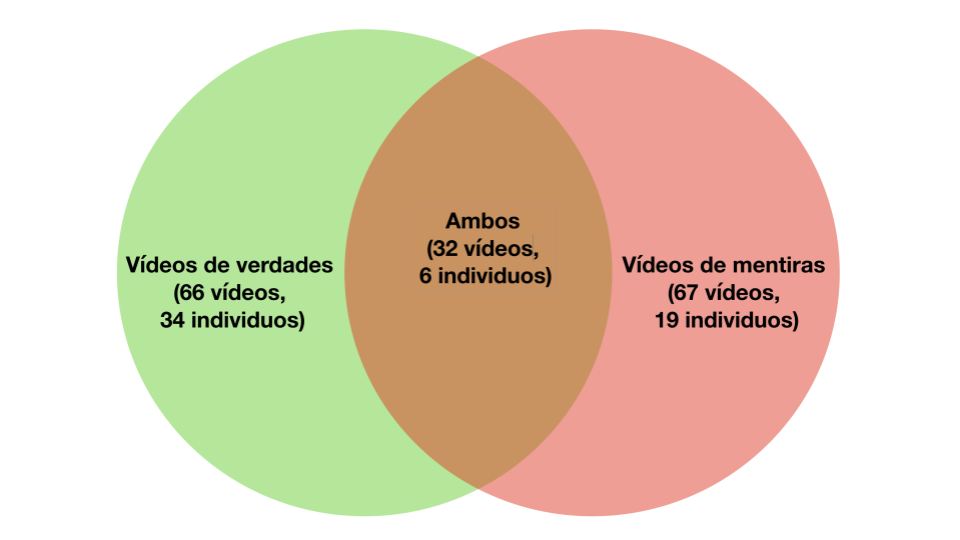
\includegraphics[width=9cm,keepaspectratio]{XX_Figures/Fig_Dataset1_Venn.png}
	\caption{\footnotesize Diagrama de Venn del dataset piloto.}
	\label{fig:Fig_Dataset1_Venn}
\end{figure}

Por la poca cantidad de videos se decidió que en el conjunto de Test hubiera personas distintas en lugar de declaraciones ya que a pesar de que varias personas aparecían en diferentes videos con diferentes declaraciones, éstas solo aparecían en una sola clase (verdad o mentira). Adicionalmente se obtuvieron más videos de los 121 videos que contenía el dataset "Trial" (Figura \ref{fig:Fig_Dataset1}), ya que algunos videos tenían lapsos de tiempo en la que el sujeto no aparecía en la escena y se dividió en un nuevo video por cada lapso nuevo en la que no aparecía el individuo; de esta manera se obtuvieron más videos y se eliminaron datos sin importancia.
En la Figura \ref{fig:Fig_Dataset1_Venn} se observa un diagrama de Venn de como están distribuidos los videos en el Dataset `Trial'. en verde se observa que se tienen 66 videos con 34 personas distintas etiquetadas como verdad, en rojo 67 videos con 19 individuos etiquetadas como mentira y en la intersección se encuentran 32 videos con 6 individuos que aparecen con la etiqueta de verdad y otros con la etiqueta de mentira.

Para el entrenamiento y pruebas de desempeño de la red, los datos se dividieron de la siguiente manera:

\begin{itemize}
    \item Train: 106 videos para los datos de entrenamiento.
    \item Validation: Este conjunto de datos se obtuvo extrayendo datos un 10 \% de los datos de Train por lo tanto contiene mismas personas que en el conjunto de Train.
    \item Test: 27 videos para los datos de prueba.  Este conjunto de datos contiene diferentes personas y declaraciones que en el conjunto de Train y Validation.
\end{itemize}

%---------------------
%---------------------
%---------------------


\subsection{Dataset `Interview'}
\label{sec:DatasetInterview}

Este nuevo conjunto de datos ha sido utilizado por su Lloyd \cite{Lloyd2019MiamiDatabase} para probar la hipótesis de que las personas tienden a juzgar de diferente manera a las razas para decidir si mienten o dicen la verdad; Las personas obtuvieron una exactitud de 54\% para detectar mentiras y verdades \cite{Lloyd2019MiamiDatabase}. La cantidad de videos que contiene es casi el triple que el anterior dataset ocupado y está más equilibrado en tiempo, videos y personas. A continuación se listan las características de este conjunto:\\


\begin{itemize}
    \item 320 videos de aproximadamente 30s de personas con declaraciones falsas y verdades. .
    \item Los datos están en formato RGB, 30 Fotogramas por segundo (30 FPS), MP4 y 1280x720.
    \item hay 80 individuos diferentes en donde 20 son hombres blancos, 20 hombres negros, 20 mujeres blancas y 20 mujeres negras. Cada individuo contiene 4 videos; 2 videos con distintas declaraciones de verdad y 2 videos con distintas declaraciones de mentira.
    \item En todos los video solo aparecen los mismos sujetos sin movimiento de la cámara.
\end{itemize}

En la Figura \ref{fig:Fig_Dataset2} se muestran 16 fotogramas extraídos de 16 videos distintos. Cada uno de los 4 fotogramas pertenecientes al mismo individuo pero a diferente video muestran el mismo fondo, la misma ropa y en general el mismo ambiente.

\begin{figure}[h!]
	\centering
	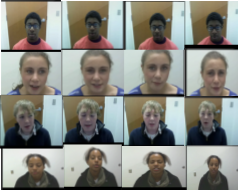
\includegraphics[width=6cm,keepaspectratio]{XX_Figures/Fig_Dataset2.png}
	\caption{\footnotesize Algunos fotogramas del Dataset `Interview'}
	\label{fig:Fig_Dataset2}
\end{figure}

En el Capítulo \ref{Chapter3} se menciona que Bashar A. Rajoub en Junio del 2014 \cite{Rajoub2014ThermalDetection}, obtuvo un pobre desempeño predictivo al segmentar los datos con la metodología \textit{leave-one-person-out} en la que los individuos de los datos de prueba eran distintos a los individuos de los datos de entrenamiento, pero obtuvo excelentes resultados con la metodología \textit{within-indidivual} en la que los individuos de los datos de entrenamiento también se encontraban en los datos de prueba pero con diferentes declaraciones.\\

Como este conjunto de datos es casi tres veces más grande que el dataset `Trial' y equilibrado en personalidades y duración, se decidió dividir los datos de prueba en TestWI y TestPO para probar si se obtenían resultados similares con las dos metodologías que Bashar A. Rajoub y otros artículos obtuvieron . Se segmentaron los datos de la siguiente manera (Figura \ref{fig:Fig_Dataset2_Segmentos}):

\begin{figure}[th]
	\centering
	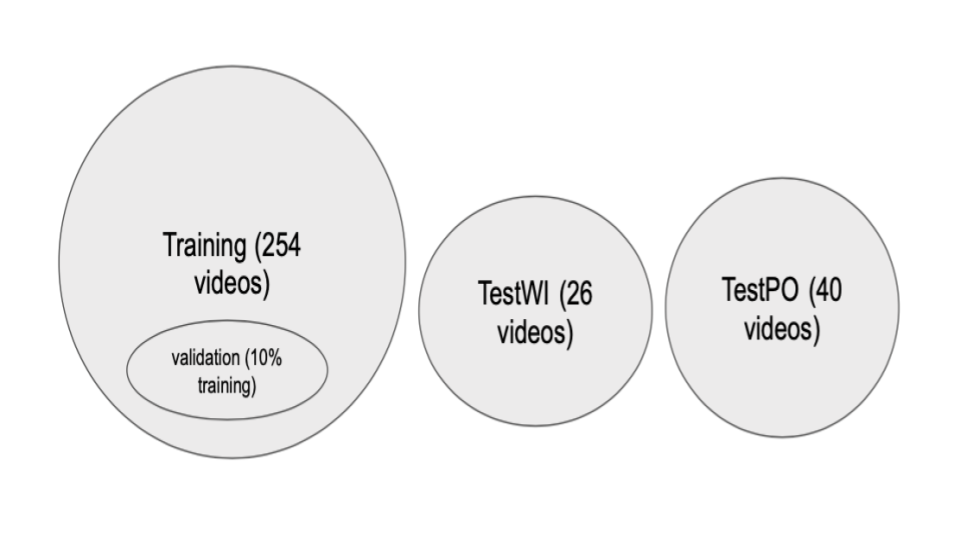
\includegraphics[width=10cm,keepaspectratio]{XX_Figures/Fig_Dataset2_Segmentos.png}
	\caption{\footnotesize Segmentos propuestos del Dataset `Interview' para los modelos propuestos.}
	\label{fig:Fig_Dataset2_Segmentos}
\end{figure}

\begin{itemize}
    \item \textbf{Train}: 254 videos (79.3\%): En la ecuación \ref{equ:Train}, se observa cómo esta compuesto el conjunto de entrenamiento. Este conjunto de entrenamiento contiene un total de 70 personas diferentes, 57 con 4 videos diferentes (2 con declaraciones de verdad y 2 de mentira) y 13 personas con 2 videos diferentes (1 de verdad y 1 de mentira)
    \begin{equation}
    \label{equ:Train}
        Train = 57_{personas} * 4_{V,V,M,M} + 13_{personas} * 2_{V,M}
    \end{equation}
    
    \item \textbf{Test within-indidivual (TestWI)}: 26 videos (8\%): En la ecuación \ref{equ:TestWI}, se observa cómo esta compuesto el conjunto de pruebas TestWI. Este conjunto de pruebas contiene 13 personas distintas y son personas que también se encuentran en el conjunto de entrenamiento pero con diferentes videos y declaraciones.
    \begin{equation}
    \label{equ:TestWI}
        TestWI = 13_{personas} * 2_{V,M}
    \end{equation}
    
    \item \textbf{Test leave-one-person-out (TestPO)}: 40 videos (12.7\%): En la ecuación \ref{equ:TestPO}, se observa cómo esta compuesto el conjunto de pruebas TestPO. Este conjunto de pruebas contiene 20 personas y son personas distintas al conjunto de entrenamiento.
    \begin{equation}
    \label{equ:TestPO}
        TestPO = 20_{personas} * 4_{V,V,M,M}
    \end{equation}
    
\end{itemize}

%---------------------------------
%---------------------------------

\section{Nomenclatura}
\label{sec:Nomenclatura}

En esta sección se explicará la nomenclatura que se ocupa para los diferentes modelos utilizados en las siguientes secciones. Algunos de estos conceptos ya se encuentran explicados en el Capítulo \ref{Chapter2}. Al comienzo de cada modelo se tendrá 3D que indica que la arquitectura está basada en redes neuronales convolucionales 3D. lo primero en aplicarle a la entrada de todos los modelos será una capa convolucional, seguida por una capa maxpooling y en caso de tener varias capas convolucionales y varias capas maxpooling, seguiran teniendo la estructura (C1,M1,C2,M3,C3,...,Cn) o (C1,M1,C2,M3,C3,...,Mn), Cn representando la capa convolocional n y Mn la n capa maxpooling. Para todos los modelos se aplicaron los filtros convolucionales a los canales por separado, por lo tanto la profundidad de canales de los kernels en todos los modelos es de 1. También se utilizo el optimizador Adam y la función de perdida Cross Entropy.

\begin{itemize}
    \item  {[ID]\textbf{DS}}: Indica el dataset que se está ocupando en el modelo y el preprocesamiento personalizado que tuvo. Los valores de DS se encuentran en la tabla \ref{tab:DS}.
    \begin{itemize}
        \item Dataset: Dataset que se está ocupando.
        \item  FrameSize: Tamaño espacial de los fotogramas.
        \item ObjectFrame: objetos que se encuentran en la mayoría de los fotogramas al terminar el preprocesamiento.
    \end{itemize}
    
    \begin{table}[h!]
    \centering
    \begin{tabular}{|c|c|c|c|}
        \hline 
        ID\_DS & Dataset & FrameSize & ObjectFrame\tabularnewline
        \hline 
        \hline 
        {[}1{]} & Trial & 100x100 & Face,shoulders,arms\tabularnewline
        \hline 
        {[}2a{]} & Interview & 50x50 & Face,shoulders,arms\tabularnewline
        \hline 
        {[}2b{]} & Interview & 50x50 & Face\tabularnewline
        \hline 
        {[}2c{]} & Interview & 100x100 & Face,shoulders,arms\tabularnewline
        \hline 
    \end{tabular}
    \caption{\footnotesize IDs de \textbf{DS}.}.
    \label{tab:DS}
    \end{table} 
    
    %----------------------------------------------------------------------------
    \item {[ID]\textbf{CH}}: Combinación de canales ocupados por el modelo. Los valores de CH se encuentran en la tabla \ref{tab:CH}.
    \begin{table}[h!]
    \centering
    \begin{tabular}{|c|c|}
        \hline 
        [ID]CH & Channels\tabularnewline
        \hline 
        \hline 
        {[}0{]} & R,G,B\tabularnewline
        \hline 
        {[}1{]} & GS,KIR,LAP\tabularnewline
        \hline 
        {[}2{]} & GS,OX,OY\tabularnewline
        \hline 
        {[}3{]} & GS,SX,SY\tabularnewline
        \hline 
        {[}4{]} & GS\tabularnewline
        \hline 
        {[}5{]} & KIR\tabularnewline
        \hline 
        {[}6{]} & SX,SY\tabularnewline
        \hline 
        {[}7{]} & OX,OY\tabularnewline
        \hline 
        {[}8{]} & GS KIR\tabularnewline
        \hline 
        {[}9{]} & GS,KIR,SX,SY\tabularnewline
        \hline 
    \end{tabular}%
    \caption{\footnotesize IDs de \textbf{CH}.}.
    \label{tab:CH}
    \end{table} 
    %-----------------------------------------------------------------
    \item {[ID]\textbf{Fr}}: Los valores de FR se encuentran en la tabla \ref{tab:Fr}.
    \begin{itemize}
        \item Frames: Indica el índice de la tabla que especifica la cantidad de fotogramas utilizados en el modelo.
        \item FramesPerConvolution: Menciona cuántos fotogramas ocupan los kernels por capa convolucional en la dimensión temporal. 
        \item FrameSpace: Se refiere a la cantidad de espacios (fotogramas) que hay entre los fotogramas seleccionados, este procedimiento se puede apreciar en la Figura \ref{fig:Fig_FrameSpace}.
        \item TemporalSride: Menciona los valores de stride en la dimensión temporal de cada capa maxpooling, un ejemplo se observa entre la Figura \ref{fig:Fig_Ejemplo_3DCNN} y  la Figura \ref{fig:Fig_3DCNN_TemporalStride}.
    \end{itemize}
    
    \begin{table}[h!]
    \centering
    \begin{tabular}{|c|c|c|c|c|}
        \hline 
        {[}ID{]}Fr & Frames & FrameSpace & FramesPerConvolution & TemporalStrides\tabularnewline
        \hline 
        \hline 
        {[}0{]} & 7 & 0 & {[}3,3,3,1,1{]} & {[}1,1,1,1{]}\tabularnewline
        \hline 
        {[}1{]} & 7 & 1 & {[}3,3,3,1,1{]} & {[}1,1,1,1{]}\tabularnewline
        \hline 
        {[}2{]} & 14 & 0 & {[}4,4,4,4,2{]} & {[}1,1,1,1{]}\tabularnewline
        \hline 
        {[}3{]} & 28 & 1 & {[}8,8,8,7{]} & {[}1,1,1{]}\tabularnewline
        \hline 
        {[}4{]} & 100 & 2 & {[}9,7,7,7{]} & {[}2,2,2,2{]}\tabularnewline
        \hline 
        {[}5{]} & 7 & 1 & {[}2,3{]} & {[}2,1{]}\tabularnewline
        \hline 
    \end{tabular}%
    \caption{\footnotesize IDs de \textbf{Fr}.}.
    \label{tab:Fr}
    \end{table} 
    %----------------------------------------------------------------------------
    
    \item {[ID]\textbf{FC}}: FeaturesPerConvolution indica el índice en la tabla para sabe cuantos kernels convolucionales se ocuparon por capa convolucional para obtener mapas de características. Los valores de FC se encuentran en la tabla \ref{tab:FC}.
    
    \begin{table}[h!]
    \centering
    \begin{tabular}{|c|c|}
        \hline 
        {[}ID{]}FC & FeaturesPerConvolution\tabularnewline
        \hline 
        \hline 
        {[}0{]} & 2,4,8,16,32\tabularnewline
        \hline 
        {[}1{]} & 2,8,32,128\tabularnewline
        \hline 
        {[}2{]} & 4,8,16,32,64\tabularnewline
        \hline 
        {[}3{]} & 4,12,36,108,217\tabularnewline
        \hline 
        {[}4{]} & 4,12,36,128,256\tabularnewline
        \hline 
        {[}5{]} & 6,12,24,48,96\tabularnewline
        \hline 
        {[}6{]} & 8,16,32,64\tabularnewline
        \hline 
        {[}7{]} & 8,16,32,64.128\tabularnewline
        \hline 
        {[}8{]} & 10,20,30,40\tabularnewline
        \hline 
        {[}9{]} & 2,3\tabularnewline
        \hline 
        {[}10{]} & 8,32,128,256,512\tabularnewline
        \hline 
        {[}11{]} & 6,32,128,256\tabularnewline
        \hline 
        {[}12{]} & 16,32,128,256\tabularnewline
        \hline 
        {[}13{]} & 4,8,16,32\tabularnewline
        \hline 
        {[}14{]} & 6,8,32,128\tabularnewline
        \hline 
        {[}15{]} & 8,16,32,64,256\tabularnewline
        \hline 
    \end{tabular}%
    \caption{\footnotesize IDs de \textbf{FC}.}.
    \label{tab:FC}
    \end{table} 
    %----------------------------------------------------------------------------
    
    \item  {[ID]\textbf{MP}}: índice de la tabla que indica las funciones de transferencia, capas y número de neuronas en la MLP. Los valores de MP se encuentran en la tabla \ref{tab:MP}.
    \begin{itemize}
        \item TransferFunctions: Indica la funciones de transferencia ocupadas en cada capa de la MLP. En el caso de las capas convolucionales, todas las funciones de transferencia son ReLu.
        \item  NeuronsPerLayer: Indica el número de neuronas por capa en la MLP
    \end{itemize}
    
    \begin{table}[h!]
    \centering
    \begin{tabular}{|c|c|c|}
        \hline 
        {[}ID{]}MP & NeuronsperLayer & TransferFunctions\tabularnewline
        \hline 
        \hline 
        {[}0{]} & 256,1024,2 & R,R\tabularnewline
        \hline 
        {[}1{]} & 192,512,2 & R,R\tabularnewline
        \hline 
        {[}2{]} & 384,512,2 & R,R\tabularnewline
        \hline 
        {[}3{]} & 651,1024,2 & R,R\tabularnewline
        \hline 
        {[}4{]} & 192,1024,2 & R,R\tabularnewline
        \hline 
        {[}5{]} & 384,1024,2 & R,R\tabularnewline
        \hline 
        {[}6{]} & 64,64,2 & R,R\tabularnewline
        \hline 
        {[}7{]} & 32,32,2 & R,R\tabularnewline
        \hline 
        {[}8{]} & 288,512 & R,R\tabularnewline
        \hline 
        {[}9{]} & 768,1024,2 & R,R\tabularnewline
        \hline 
        {[}10{]} & 240,512 & R,R\tabularnewline
        \hline 
        {[}11{]} & 18,10,2 & R,R\tabularnewline
        \hline 
        {[}12{]} & 768,512,2 & R,R\tabularnewline
        \hline 
        {[}13{]} & 64,32,2 & R,R\tabularnewline
        \hline 
        {[}14{]} & 512,1024,2 & R,R\tabularnewline
        \hline 
        {[}15{]} & 3072,4096,2 & R,R\tabularnewline
        \hline 
        {[}16{]} & 768,128,128,128,128,128,128,128,128,128,2 & R,R,R,R,R,R,R,R,R,R\tabularnewline
        \hline 
        {[}17{]} & 96,1024,1024,1024,1024,1024,1024,1024,1024,1024,2 & T,R,R,R,R,R,R,R,R,R\tabularnewline
        \hline 
        {[}18{]} & 384,128,128,128,128,128,128,128,64,32,2 & T,R,R,R,R,R,R,R,R,R\tabularnewline
        \hline 
        {[}19{]} & 768,1024,1024,2 & R,R,R\tabularnewline
        \hline 
        {[}20{]} & 288,1024,2 & R,R\tabularnewline
        \hline 
        {[}21{]} & 128,128,128,128,128,128,128,128,64,32,2 & T,R,R,R,R,R,R,R,R,R\tabularnewline
        \hline 
        {[}22{]} & 512,128,128,128,128,128,128,128,128,128,2 & R,R,R,R,R,R,R,R,R,R\tabularnewline
        \hline 
        {[}23{]} & 256,128,128,128,128,128,128,128,128,128,2 & R,R,R,R,R,R,R,R,R,R\tabularnewline
        \hline 
    \end{tabular}%
    \caption{\footnotesize  IDs de \textbf{MP}.}.
    \label{tab:MP}
    \end{table} 
    
    %----------------------------------------------------------------------------
    
    \item  {[n/DV]\textbf{DO}}: n indica el porcentaje de dropout utilizado en el modelo. El Dropout es una técnica en la que neuronas seleccionadas al azar se ignoran durante el entrenamiento (se desconectan al azar). A medida que una red neuronal aprende, los pesos de las neuronas se ajustan para características específicas que proporcionan cierta especialización. Las neuronas vecinas empiezan a confiar en esta especialización, que si se lleva demasiado lejos puede dar como resultado un modelo frágil demasiado especializado para los datos de entrenamiento. Al agregar el dropout y así eliminar neuronas aleatoriamente, otras neuronas tendrán que intervenir y manejar la representación requerida para hacer predicciones para las neuronas que han sido desconectadas dando como resultado que la red aprenda múltiples representaciones internas independientes. En el caso se ser DV significa que se ocupa el concepto Dropout Variable en él. Dropout variable es una propuesta para solucionar el problema del sobreajuste  (overfitting) que puede llegar a existir en los modelos y consiste en aumentar la probabilidad de desconexión de las neuronas cuando el modelo comienza a obtener un accuracy mayor al 60\% en el conjunto de entrenamiento.
    
     \item  {[ID]\textbf{LR}}: indica la tasa de aprendizaje (Learning Rate) que controla cuánto se deben ajustar los pesos de la red neuronal con respecto al gradiente. Cuanto más bajo es el valor, más lento viajamos a lo largo de la pendiente descendente. Los valores de LR se encuentran en la tabla \ref{tab:LR}.
     \begin{table}[h!]
        \centering
        \begin{tabular}{|c|c|c|}
            \hline 
            {[}ID{]}LR & Learning Rate\tabularnewline
            \hline 
            \hline 
            {[}0{]} & 0.01\tabularnewline
            \hline 
            {[}1{]} & 0.001\tabularnewline
            \hline 
            {[}2{]} & 0.0001\tabularnewline
            \hline 
        \end{tabular}%
        \caption{\footnotesize  IDs de \textbf{LR}.}.
        \label{tab:LR}
      \end{table} 
     
      \item  {[ID]\textbf{BS}}: indica el tamaño de lote (Batch size) el cual se refiere a la cantidad de muestras de entrenamiento que se propagarán a través de la red. Los valores de BS se encuentran en la tabla \ref{tab:BS}.
      \begin{table}[h!]
        \centering
        \begin{tabular}{|c|c|c|}
            \hline 
            {[}ID{]}BS & Batch Size\tabularnewline
            \hline 
            \hline 
            {[}0{]} & 100\tabularnewline
            \hline 
            {[}1{]} & 150\tabularnewline
            \hline 
            {[}2{]} & 200\tabularnewline
            \hline 
            {[}3{]} & 300\tabularnewline
            \hline 
            {[}4{]} & 500\tabularnewline
            \hline 
        \end{tabular}%
        \caption{\footnotesize  IDs de \textbf{BS}.}.
        \label{tab:BS}
      \end{table} 
    %----------------------------------------------------------------------------
\end{itemize}

Un ejemplo de un modelo utilizando esta nomenclatura se muestra a continuación.\\

\textbf{3D-[1]DS-[0]CH-[5]Fr-[9]FC-[11]MP-[50]DO-[1]LR-[4]BS}\\
 
 \begin{itemize}
     \item {[1]DS}: Tener 1 Tabla \ref{tab:DS} indica que se está ocupando el dataset `Trial' con fotogramas redimensionados a 100x100 píxeles y en los fotogramas aparecen los rostros, hombros y brazos de las personas.
     \item {[0]CH}: Al tener 0 en el índice de la tabla \ref{tab:CH}, indica que este modelo ocupa los canales R,G,B. La separación de los canales se observa en la Figura \ref{fig:Fig_CH}.
     \begin{figure}[h!]
    	\centering
    	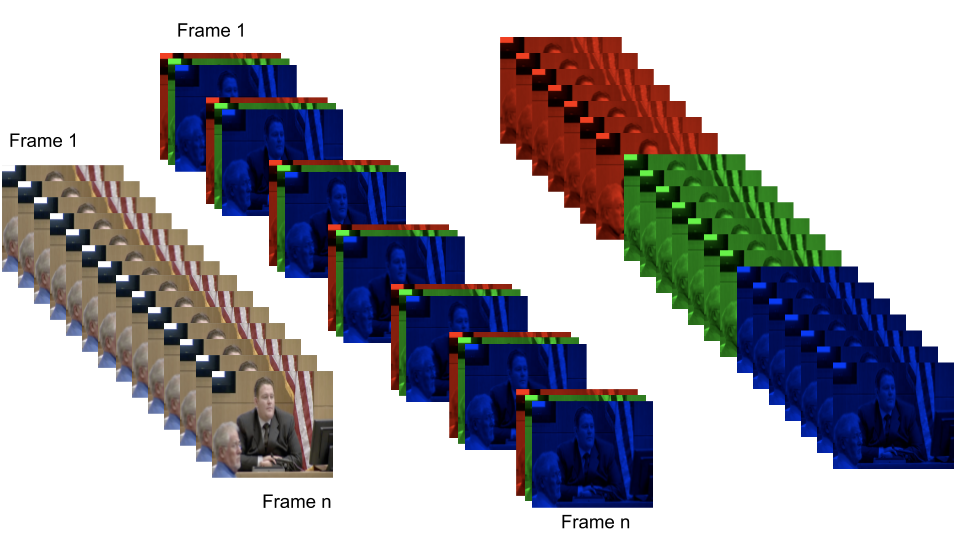
\includegraphics[width=9cm,keepaspectratio]{XX_Figures/Fig_Fr.png}
    	\caption{\footnotesize CH}
    	\label{fig:Fig_CH}
    \end{figure}
     \item {[5]Fr}: Al tener 5 en el índice de la tabla \ref{tab:Fr}, indica que este modelo ocupa como entrada 7 fotogramas. FrameSpace 1 indica que en el preprocesamiento de los fotogramas se tomaron los fotogramas saltándose un fotograma como se muestra en la figura \ref{fig:Fig_Fr}. [2,3] FramesPerConvolution indica que por cada capa convolucional (2 capas totales), los kernels tendrán una profundidad temporal de 2 en la primera capa y 3 en la s capa. [2,1] TemporalStrides indica que el paso en la dimensión temporal por cada capa maxpooling es de 1.
     \begin{figure}[h!]
    	\centering
    	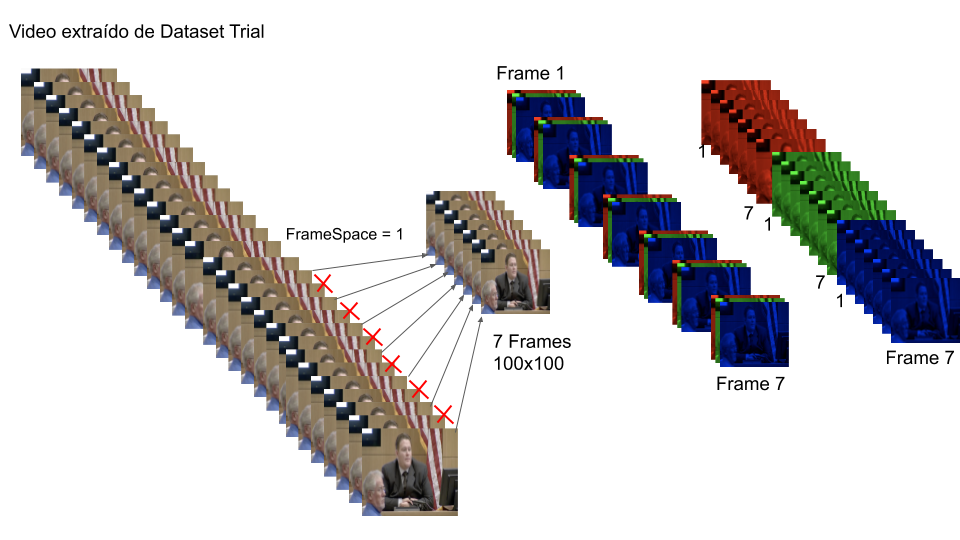
\includegraphics[width=11cm,keepaspectratio]{XX_Figures/Fig_CH.png}
    	\caption{\footnotesize  Fr}
    	\label{fig:Fig_Fr}
    \end{figure}
     \item {[9]FC}: Al tener 9 en el índice de la tabla \ref{tab:FC}, indica la cantidad de kernels que hay por capa convolucional. Se tendrían 2 kernels para la primera capa, 3 para la última capa como se muestra en la figura \ref{fig:Fig_FrFC}.
     \begin{figure}[h!]
    	\centering
    	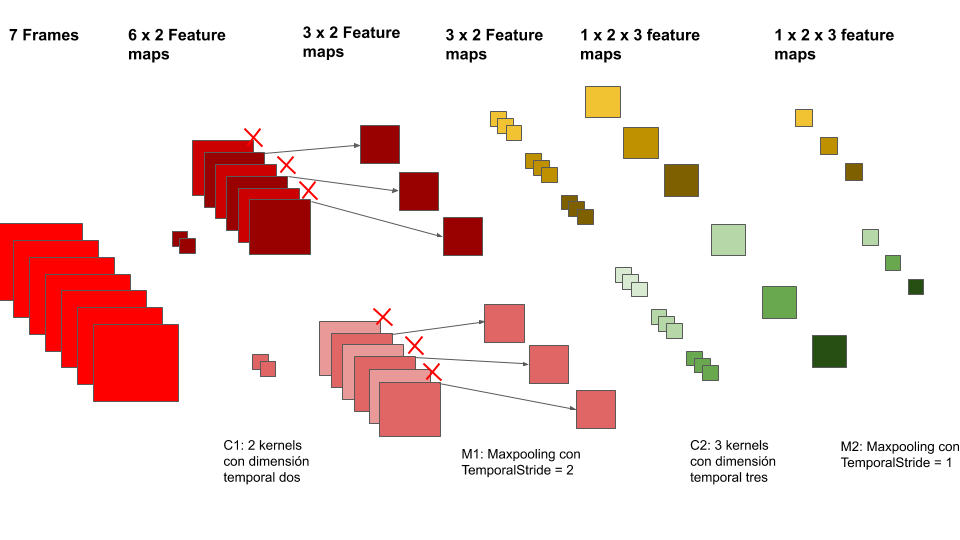
\includegraphics[width=13cm,keepaspectratio]{XX_Figures/Fig_FrFC.png}
    	\caption{\footnotesize  Fr y FC}
    	\label{fig:Fig_FrFC}
    \end{figure}
     \item {[11]MP}: Al tener 11 en el índice de la tabla \ref{tab:MP}, indica que se tendrán 3 capas en la MLP, la primera con 18 neuronas y una función de activación ReLu, la segunda con 5 neuronas y función de activación ReLu; y la última capa con dos neuronas sin función de activación como se muestra en la figura \ref{fig:Fig_MP}.
     \begin{figure}[h!]
    	\centering
    	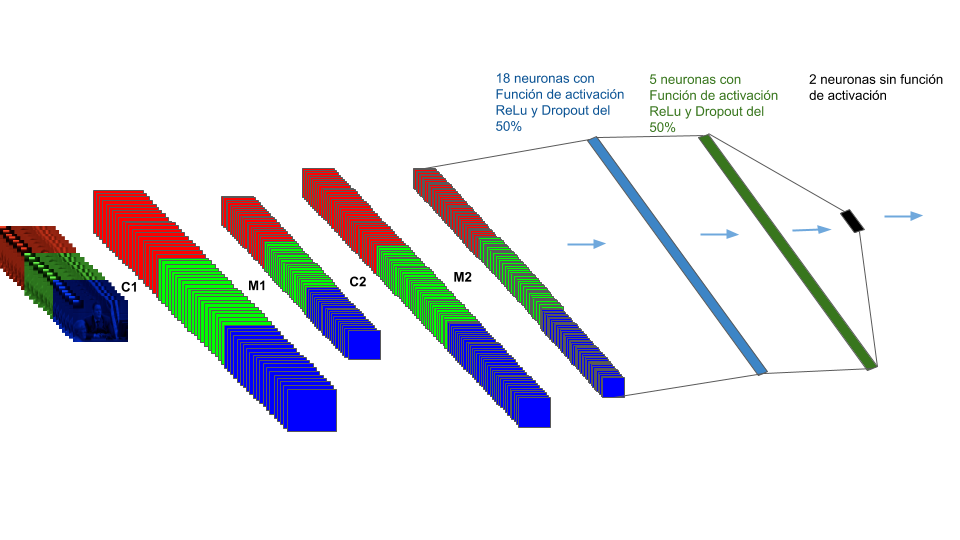
\includegraphics[width=15cm,keepaspectratio]{XX_Figures/Fig_MP.png}
    	\caption{\footnotesize  MP}
    	\label{fig:Fig_MP}
    \end{figure}
     \item {[50]DO}: indica que las neuronas en la MLP tienen una probabilidad de desconexión del 50\% (Dropout 50\%).
     \item {[1]LR}: indica que se está ocupando una tasa de aprendizaje de 0.01 para el optimizador Adam.
     \item {[4]BS}: indica que el tamaño del lote (batch size) es de 500 datos para el entrenamiento.
 \end{itemize}
 

%----------------------------------------------------------------------------------------
%----------------------------------------------------------------------------------------
%----------------------------------------------------------------------------------------
\section{Modelos pilotos}
\label{sec:Modelos_pilotos}

En el capítulo \ref{Chapter3} se mencionó algunos de los trabajos que han tratado de detectar mentiras con el uso de diferentes sistemas computacionales. El modelo piloto que se propone se basó en la arquitectura de red que se menciona en  \cite{Ji20133DRecognition} en la que se lograron clasificar correctamente acciones humanas en videos y en \cite{KrishnamurthyADetection} clasificaron mentiras y verdades en videos. \\

Se utilizó la métrica \textit{AccuracyData} (Ecuación \ref{equ:Accuracy}) para evaluar el modelo. 

\subsection{Modelo piloto}
\label{sec:Modelo3D7F}

\subsubsection{Descripción del Modelo}
\label{sec:DescripcionModeloPiloto}

 Nomenclatura Modelo piloto:\\ \textbf{3D-[1]DS-[0]CH-[0]Fr-[15]FC-[19]MP-[50]DO-[1]LR-[4]BS}\\

Según la nomenclatura propuesta, la arquitectura de red consiste:\\

\begin{itemize}
    \item {[1]DS}
        \begin{itemize}
            \item Dataset utilizado `Trial'
            \item Imágenes de 100 x 100 en la que aparece el rostro, hombros y brazos de una persona.
    \end{itemize}
    
    \item {[0]CH}
        \begin{itemize}
            \item Canales RGB
    \end{itemize}

    \item {[0]Fr}
        \begin{itemize}
            \item Datos de 7 fotogramas.
            \item FrameSpace 1
            \item Frames per Convolution (3,3,3,1,1)
            \item TemporalStride (1,1,1,1)
    \end{itemize}
    
    \item {[15]FC}
        \begin{itemize}
            \item Features per Convolution (8,16,32,64,256)
    \end{itemize}
    
    \item {[19]MP}
        \begin{itemize}
            \item 768 neuronas en la capa de entrada de la MLP con función de activación ReLu, 1024 en las capas ocultas con función de activación ReLu y 2 en la capa de salida con función SoftMax.
    \end{itemize}
    
    \item {[50]DO}
        \begin{itemize}
            \item Dropout 50\%
            
    \item {[1]LR}: indica que se está ocupando una tasa de aprendizaje de 0.01 para el optimizador Adam.
    
     \item {[4]BS}: indica que el tamaño del lote (batch size) es de 500 datos para el entrenamiento.
    \end{itemize}

\end{itemize}


%Es importante resaltar que el conjunto de Test es la que mostrará que tan confiable es el sistema para detectar mentiras. Es por eso que para lograr que nuestro modelo se enfoque en la tarea de detectar mentiras y no en la memorización de los individuos, es necesario que existan declaraciones o personas  distintas en el conjunto del Train y en el conjunto de Test. 


\subsubsection{Análisis de desempeño}
\label{sec:TDesempenoModeloPiloto}

%El modelo fue programado y probado en Python, utilizando la biblioteca de código abierto Tensorflow, desarrollado por Google para poder construir y entrenar redes neuronales. Se ocupó el Optimizador Adam  y la función de perdida Cross entropy.\\

Se tiene un total de 1658 datos para las pruebas y 10688 para los datos de entrenamiento, de los cuáles 5254 datos están etiquetados como verdad y 5434 como mentira. Cada dato es de 7 fotogramas.\\

\begin{table}[h!]
\centering
    \begin{tabular}{c c c c}
         \hline
         \textbf{Modelo} & \textbf{Train} & \textbf{Val} & \textbf{Test}\\
         \hline
         Modelo Piloto & 96\% & 95\% & 28\%\\
         \hline
    \end{tabular}
    \caption{\footnotesize  Desempeño del modelo piloto.}.
    \label{tab:TModeloPiloto}
\end{table}

En la tabla \ref{tab:TModeloPiloto} se muestran los resultados obtenidos por el modelo piloto. A pesar de que el accuracyData del Train y Validation fue mayor al 90\%, el Test obtuvo un accuracyData del 28\%. Esto se puede deber a que los parámetros de la red están siendo sobreajustados (overfitting) a los datos de entrenamiento.\\

El sobreajuste es un problema que se puede presentar cuando se excede algún tamaño óptimo de red neuronal artificial dado un conjunto de datos determinado. Se ha demostrado que si se tiene gran cantidad de neuronas en las capas ocultas, tiene como consecuencia que la red memorice los datos de entrenamiento, causando que el accuracy en los datos de entrenamiento suba considerablemente \cite{Tetko1995Neural1.}.\\

La presencia de capas ocultas en las redes neuronales profundas hace que los modelos basados en éstos, sean propensos a un sobreajuste severo y éste puede convertirse en un reto mayor si se tiene un modelo de red neuronal con gran cantidad de parámetros y una pequeña cantidad de datos \cite{Tabares2013ImprovingDropout}, algunas opciones para evitarlo es a través de la reducción de los parámetros de la red, tener un conjunto de datos mayor o terminar el proceso de entrenamiento cuando los datos de validación empiecen a mostrar un peor desempeño \cite{Caruana2001OverfittingStopping}.\\

El proceso de entrenamiento puede llevar a la red neuronal a que sea capaz de generalizar un concepto para que cuando se presenten nuevos datos, éste sea capaz de comprenderlo y devolver un resultado fiable. Si el conjunto de datos de entrenamiento es limitado, entonces el modelo no será capaz de generalizar debido a que la red se ajustará a casos particulares del conjunto de entrenamiento y será incapaz de reconocer nuevos datos de entrada, causando sobreajuste.\\

Una manera de diagnosticar correctamente el sobreajuste es cuando el accuracy de la muestras del Train sigue incrementando mientras que el accuracy con muestras nuevas (Test) va empeorando. Este comportamiento se observa en la Figura \ref{fig:Fig_ModeloPilotoAccuracy} en la que se presentan las gráficas de accuracyData obtenido por el modelo piloto. \\

\begin{figure}[h!]
	\centering
	\includegraphics[width=14cm,keepaspectratio]{XX_Figures/Fig_3DRGB_{7F}[0]_accuracy.png}
	\caption{\footnotesize Sobreajuste en el modelo piloto}
	\label{fig:Fig_ModeloPilotoAccuracy}
\end{figure}

Existen varias formas de poder combatir el sobreajuste (overfitting), a continuación se enlistan algunas de las más comunes:

\begin{itemize}
    \item Regularización: La regularización es un proceso que limita el aprendizaje del modelo para reducir el sobreajuste. La forma más utilizada de regularización en aprendizaje profundo es a través del Dropout.
    \item Balanceo de Clases: Clases variadas y equilibradas en cantidad. Si el número de muestras no está balanceado puede causar que el modelo tienda a favor de alguna clase dominante al momento de evaluar el modelo.
    \item Configuración de Parámetros: Reducir o aumentar el número de capas y neuronas que contiene la red.
    \item Reducción de características: Reducir la cantidad de características extraídas para entrenar el modelo.
    \item Incrementar los datos: Obtener más conjuntos de datos para el entrenamiento y pruebas. Esto puede ayudar a que la red tenga suficientes muestras para generalizar y no aprender de memoria los datos con los que fue entrenado.
\end{itemize}

El modelo piloto a pesar de contener regularización por Dropout con una probabilidad del 50\% de conexión, no logró combatir el sobreajuste.\\

Al tener 5254 datos etiquetados como verdad y 5434 como mentira en el entrenamiento, no se da el caso de un desbalanceo en los datos.\\

Se tiene la hipótesis de que el exceso de dimensiones de la red o de extracción de características esté causando sobreajuste.\\


\begin{table}[h!]
\centering
    \begin{tabular}{|c|c|c|c|}
        \cline{3-4} \cline{4-4} 
        \multicolumn{1}{c}{} &  & \multicolumn{2}{c|}{Predicted}\tabularnewline
        \cline{3-4} \cline{4-4} 
        \multicolumn{1}{c}{} &  & Deceit & Truth \tabularnewline
        \hline 
        \multirow{2}{*}{Real} & Deceit & 130 & 262\tabularnewline
        \cline{2-4} \cline{3-4} \cline{4-4} 
         & Truth & 930 & 336\tabularnewline
        \hline 
    \end{tabular}
    \caption{\footnotesize  Matriz de confusión del modelo piloto.}.
    \label{tab:MCModeloPiloto}
\end{table}

En la Tabla \ref{tab:MCModeloPiloto}, se observa la matriz de confusión obtenida en las pruebas por el modelo.  El 64\% de los datos (1060 datos) fueron etiquetados como mentira al evaluar nuestro sistema por la red y 36\% como mentira. A pesar de que la matriz indica que el modelo está tendiendo a clasificar los datos como verdad, los datos de pruebas no están completamente balanceados, ya que se tienen 1266 datos con etiqueta de verdad y 392 con etiqueta de mentira. Esto puede causar confusión al evaluar el modelo y creer que la red está clasificando hacia una clase dominante. Se quitaron datos de prueba para contener un mismo número de muestras en las dos clases y se volvió a entrenar el modelo.\\

\begin{table}[h!]
\centering
    \begin{tabular}{|c|c|c|c|}
        \cline{3-4} \cline{4-4} 
        \multicolumn{1}{c}{} &  & \multicolumn{2}{c|}{Predicted}\tabularnewline
        \cline{3-4} \cline{4-4} 
        \multicolumn{1}{c}{} &  & Deceit & Truth \tabularnewline
        \hline 
        \multirow{2}{*}{Real} & Deceit & 98 & 334\tabularnewline
        \cline{2-4} \cline{3-4} \cline{4-4} 
         & Truth & 268 & 156\tabularnewline
        \hline 
    \end{tabular}
    \caption{\footnotesize  Matriz de confusión del modelo piloto con clases balanceadas.}.
    \label{tab:MCModeloPilotoB}
\end{table}

La matriz de confusión con las pruebas balanceadas (857 datos) mostrada en la tabla \ref{tab:MCModeloPilotoB} indica que la red tiende ligeramente a clasificar hacia la clase verdad a pesar de tener muestras balanceadas en las pruebas pero no hay una inclinación considerable hacia una clase dominante.\\
 
En un análisis superficial se notó que existían ciertas similitudes en los datos de entrenamiento y los datos de prueba como la pose del individuo, el enfoque de la cámara, lugar en la que se encuentra el individuo, entre otros. Estas similitudes eran muy particulares de esos videos y no se contenían en los demás. Esto puede causar que la red esté aprendiendo características particulares de los videos de entrenamiento y al tener similitud con algún dato del conjunto de pruebas daba como consecuencia un etiquetado erróneo. En la Figura \ref{fig:EtiquetadoErroneo}, se muestra este fenómeno en la que los videos de la izquierda fueron usados en el conjunto de entrenamiento y están etiquetados como verdad; los videos de la derecha fueron utilizados para el conjunto de pruebas y obtuvieron una clasificación errónea. Esto pudo haber sucedido por la similitud con los videos de entrenamiento.\\

\begin{figure}[th]
	\centering
	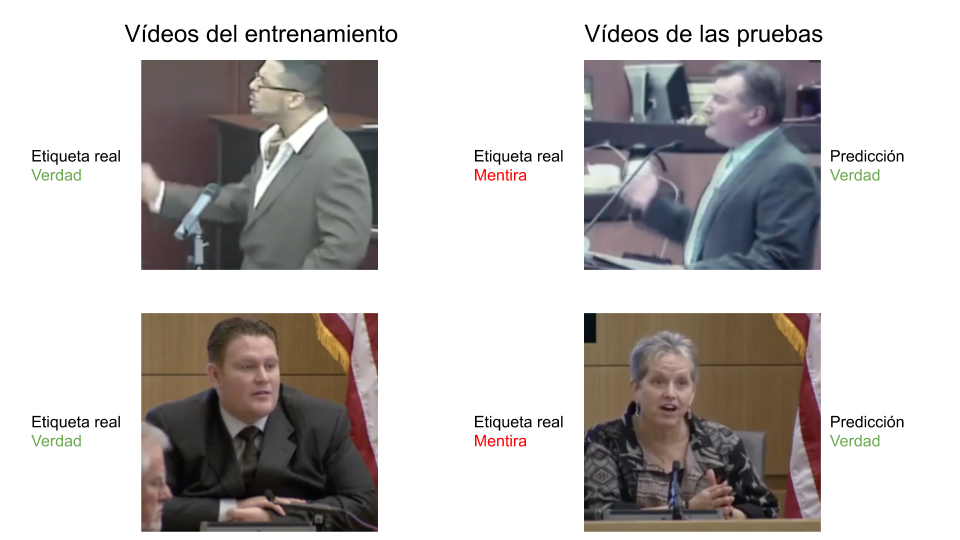
\includegraphics[width=14cm,keepaspectratio]{XX_Figures/EtiquetadoErroneo.png}
	\caption{\footnotesize Similitud entre los videos de entrenamiento y de prueba.}.
	\label{fig:EtiquetadoErroneo}
\end{figure}

A pesar de que este fenómeno se presentó en algunos datos, es difícil identificar un patrón que muestre la razón por la cuál fueron etiquetados erróneamente los demás datos de prueba.\\ 

Analizando los datos de 7 fotogramas manualmente, se encontró que la mayoría de los datos etiquetados como verdad o mentira no contenían una declaración completa de verdad o mentira como se muestra en la Figura \ref{fig:TextoFragmento7Frames}. Se tiene la hipótesis de que existen gran cantidad de fragmentos de 7 fotogramas en un video que no contienen al menos una pista que delate mentira o verdad. Esto puede causar que el modelo obtenga malos resultados al momento de clasificar verdades y mentiras por la poca información que recibe. A pesar esto, el modelo en el conjunto de entrenamiento obtuvo un accuracyData del 96\%, por lo que esta no es la causa principal del overfitting, pero puede ser factor que afecte más adelante ya que se logre solucionar el overfitting.\\ 

\begin{figure}[th]
	\centering
	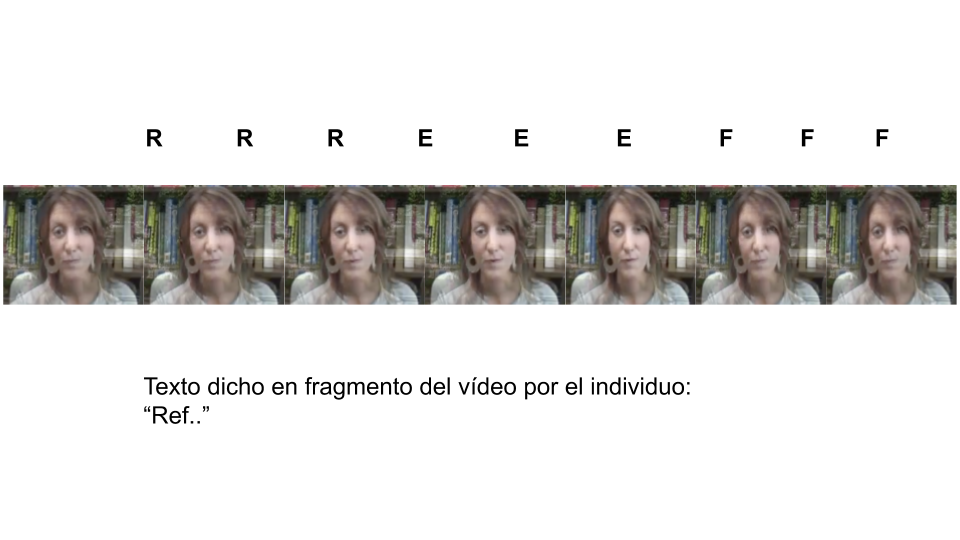
\includegraphics[width=14cm,keepaspectratio]{XX_Figures/TextoFragmento7Frames.png}
	\caption{\footnotesize Dato de 7 fotogramas con información irrelevante.}.
	\label{fig:TextoFragmento7Frames}
\end{figure}

%Una razón de esto es que el modelo se está sobre-entrenando (overfitting) y el algoritmo de aprendizaje esta siendo ajustado a ciertas características muy específicas del conjunto de datos del Train y Validation; el Test al ser un conjunto distinto muestra un desempeño diferente.

%En la Figura \ref{fig:Fig_3DRGB[0]_LossTrain} se muestra la función de costo la cual describe qué tan lejos está el resultado producido por la red del resultado esperado; en otras palabras indica la magnitud del error que el modelo cometió en la predicción. Se observa que el error producido por la red llego cero, por esta razón se alcanzó un accuracy del 100\% en los datos de Train y  Validation, mientras que en la Figura \ref{fig:Fig_3DRGB[0]_LossTest} se observa que el error en los datos aumenta considerablemente en los datos de Test, esto indica la presencia de un overfitting en nuestro modelo.

%Tener datos de 7 frames causa la problemática de que en los datos contienen poca información y no se tenga una declaración de mentira o verdad. Analizando manualmente los datos de entrada, se percató de que había datos posiblemente basura en las que no existía ningún movimiento del individuo y mucho menos se terminaba alguna declaración completa por el individuo. \\


\subsubsection{Problemáticas}
\label{sec:ProblematicasModeloPiloto}

Las problemáticas de este modelo se listan en la tabla \ref{tab:ProblematicasPiloto} y tiene el Id \textbf{1A}.

\begin{table}[th]
\centering
    \begin{tabular}{|p{1cm}|p{3cm}|p{4cm}|p{8cm}|}
        \hline 
        Id & Problemática & Posibles causas & Descripción\tabularnewline
        \hline 
        \hline 
        \multirow{3}{*}{1A} & \multirow{2}{*}{Overfitting} & Gran cantidad de parámetros & La arquitectura tiene los parámetros suficiente para memorizar los
        datos de entrenamiento.\tabularnewline
        \cline{2-4} \cline{3-4} \cline{4-4} 
         & Etiquetado Erróneo & Poca información & 7 fotogramas (1/4s) es muy poca información para contener una mentira
        o una verdad.\tabularnewline
        \hline 
    \end{tabular}
    \caption{\footnotesize  Causas de Overfitting del modelo piloto.}.
    \label{tab:ProblematicasPiloto}
\end{table}

%---------------------------------
%---------------------------------

\subsection{Variantes del modelo piloto Dataset `Trial'}
\label{sec:VariantesModeloPiloto}

\begin{figure}[p]
    	\centering
    	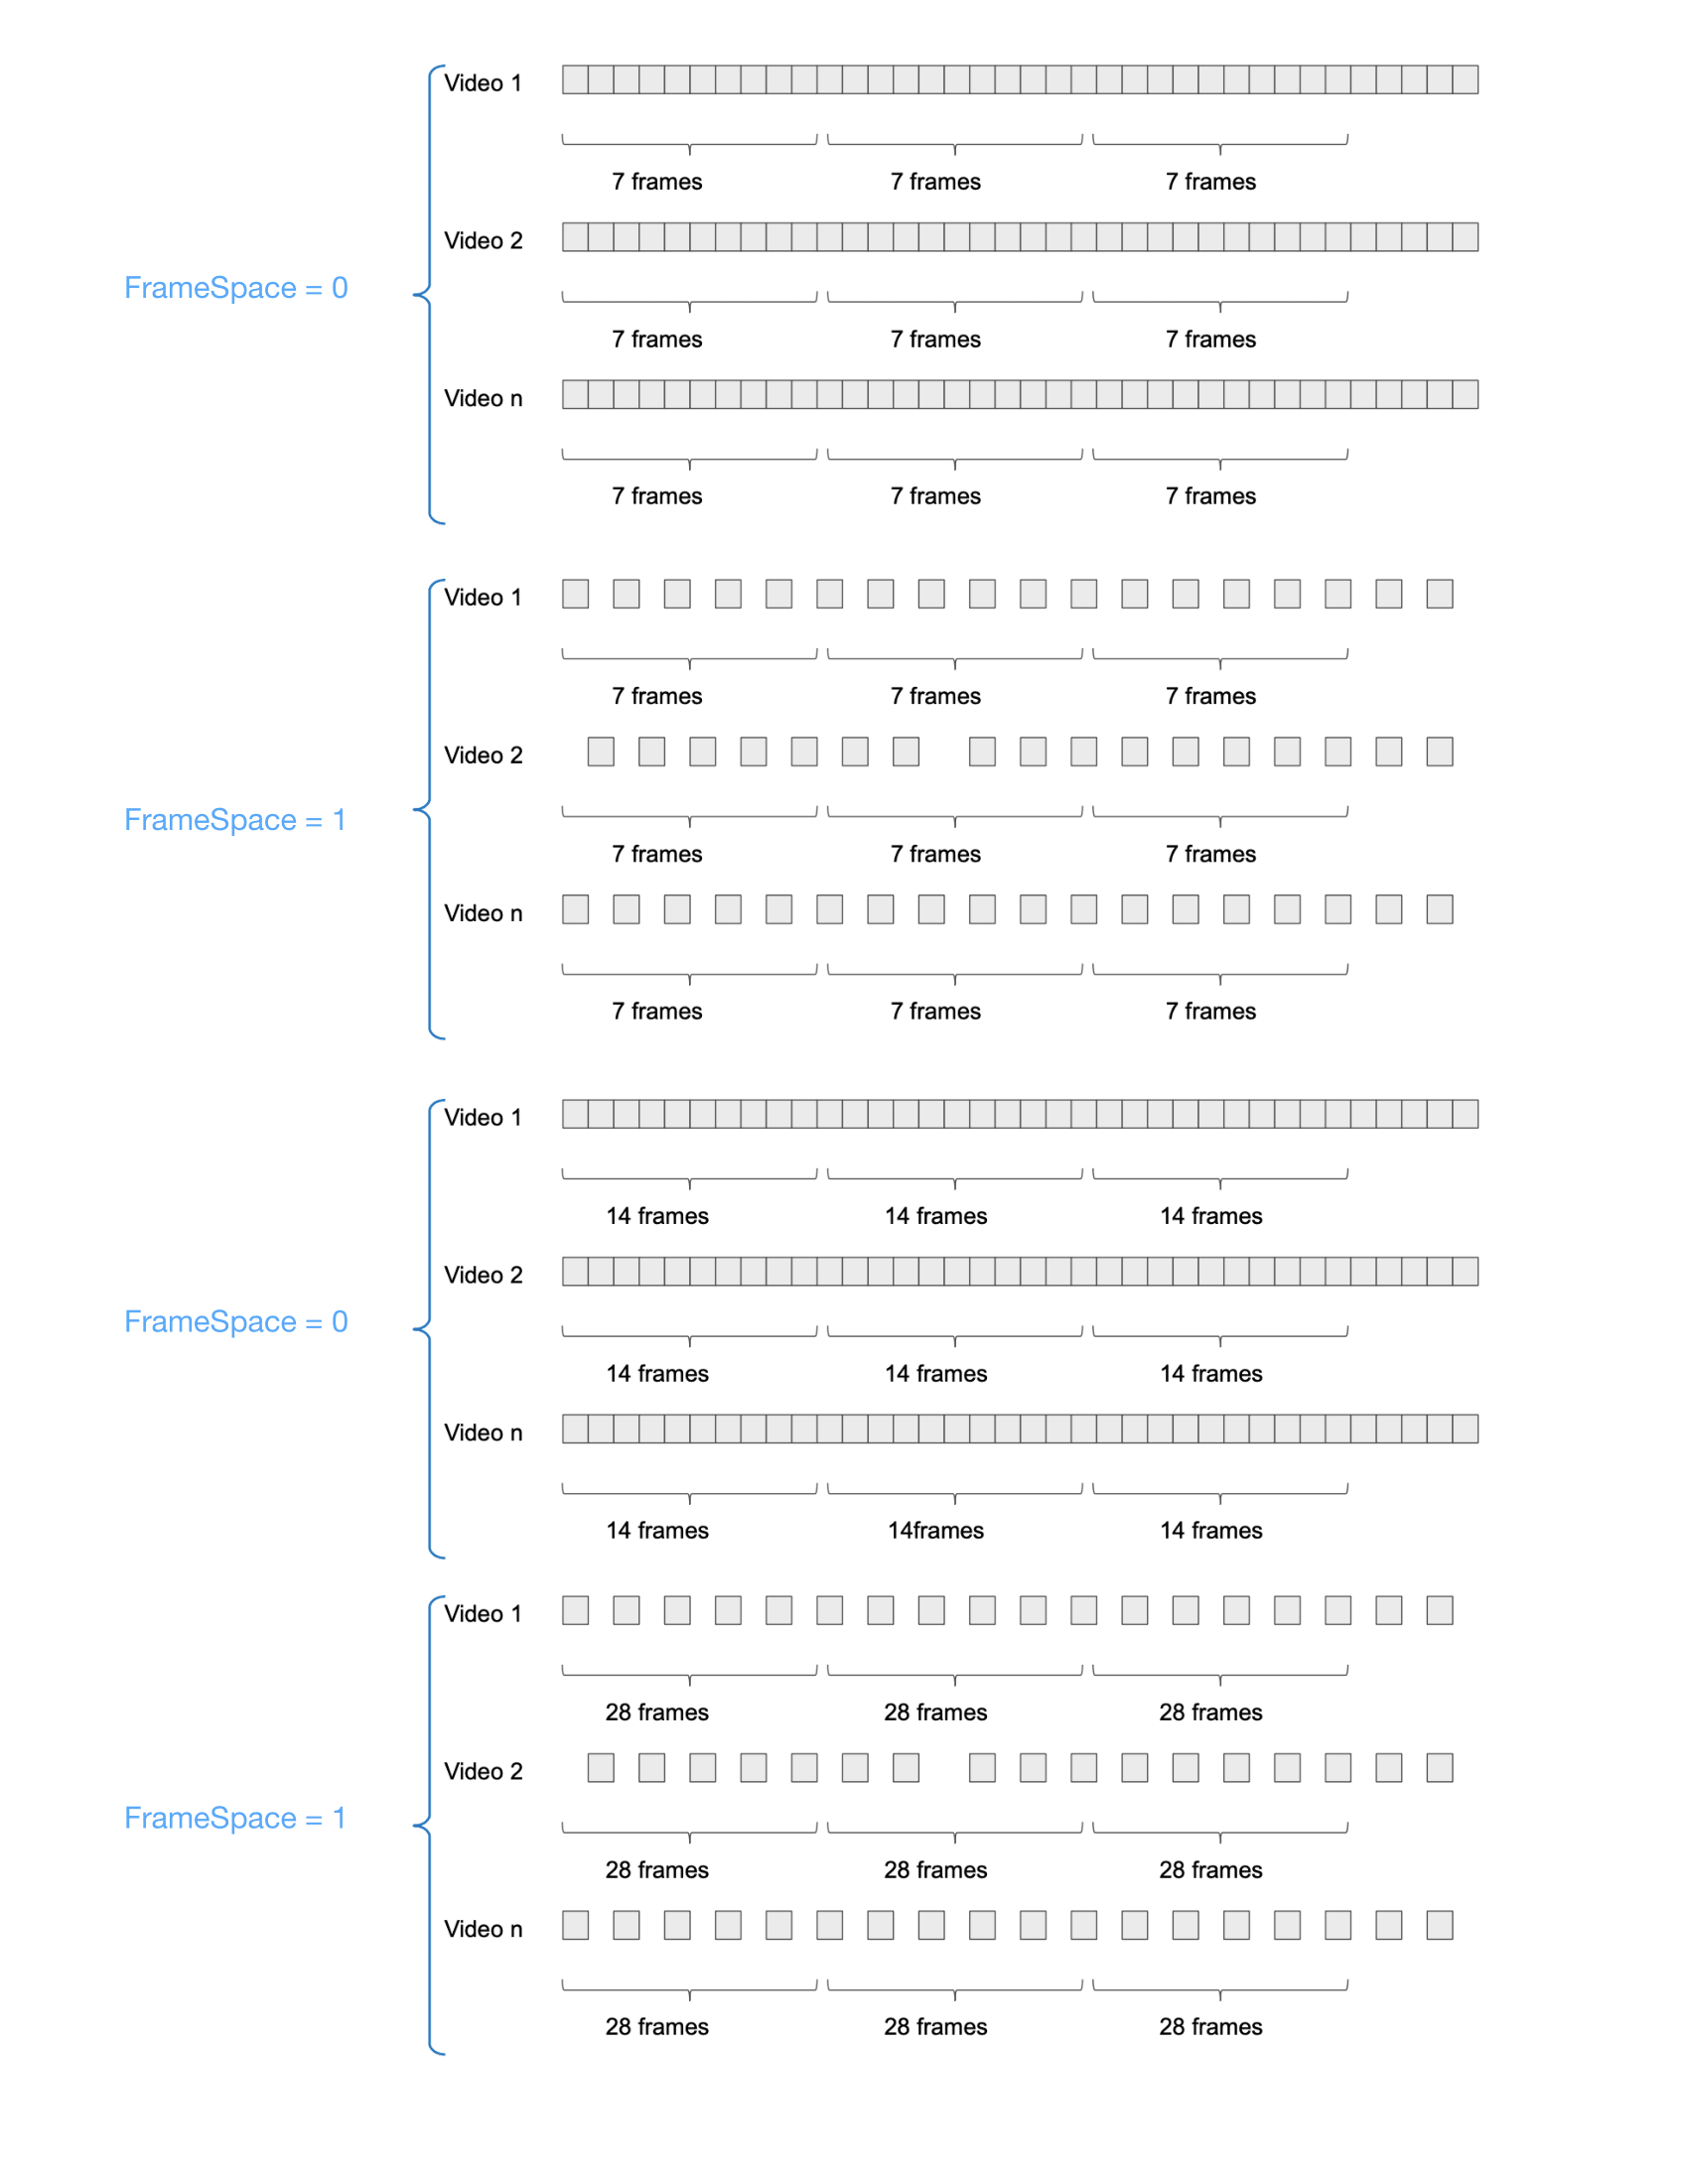
\includegraphics[width=18cm,keepaspectratio]{XX_Figures/Fig_Dataset1_7_14_28F.png}
    	\caption{\small División de los videos en datos de 7, 14 y 28 fotogramas con diferente FrameSpace.}
    	\label{fig:Fig_Dataset1_7_14_28F}
\end{figure}

Estas variantes tienen el objetivo combatir el sobreajuste con la hipótesis propuesta en la que se menciona que al extraer menor cantidad de características y tener menor cantidad de parámetros en la red ayuda a combatir el sobreajuste.\\

Para el preprocesamiento de los datos se tomaron más cantidad de fotogramas en un lapso de tiempo más grande a través del FrameSpace para observar si el comportamiento de la red cambia cuándo se tienen más movimientos del individuo y más palabras dichas por el individuo. Esta división de los datos se muestra en la Figura \ref{fig:Fig_Dataset1_7_14_28F}

\subsubsection{Descripción Modelo}
\label{sec:DescripcionVariantesModeloPiloto}

Se realizaron varios modelos de arquitecturas 3D con diferentes entradas de frames, canales, etc, y diferentes hiperparámetros de la red convolucional 3D y la MLP. Al ser gran cantidad de modelos, estos se pueden encontrar en \cite{Mendieta2019} para consultar las diferentes variantes de los modelos.
Para esta sección se seleccionaron 3 de los modelos más representativos de las pruebas.\\


%Modelo \textbf{3D-[1]DS-[2]CH-[1]Fr-[2]FC-[1]MP-[50]DO}\\

%Modelo \textbf{3D-[1]DS-[3]CH-[2]Fr-[2]FC-[12]MP-[50]DO}\\

%Modelo \textbf{3D-[1]DS-[4]CH-[3]Fr-[6]FC-[13]MP-[50]DO}\\

%---------------------------------------------------
\subsubsection{Tabla de desempeño}
\label{sec:R_3DDNN-7-14-28F-MultiChannels FS}

\begin{table}[h!]
\centering
    \begin{tabular}{|c|c|c|c|}
        \hline 
        Modelo & Train & Val & Test\tabularnewline
        \hline 
        \hline 
        3D-{[}1{]}DS-{[}2{]}CH-{[}1{]}Fr{[}2{]}FC-{[}1{]}MP-{[}50{]}DO-{[}2{]}LR-{[}4{]}BS & 96\% & 95\% & 25\%\tabularnewline
        \hline 
        3D-{[}1{]}DS-{[}3{]}CH-{[}2{]}Fr-{[}7{]}FC-{[}5{]}MP-{[}50{]}DO-{[}2{]}LR-{[}3{]}BS & 100\% & 100\% & 25\%\tabularnewline
        \hline 
        3D-{[}1{]}DS-{[}4{]}CH-{[}3{]}Fr-{[}6{]}FC-{[}13{]}MP-{[}50{]}DO-{[}2{]}LR-{[}2{]}BS & 97\% & 96\% & 33\%\tabularnewline
        \hline 
    \end{tabular}
    \caption{\footnotesize  Tres variantes del modelo piloto utilizando Dataset `Trial'.}.
    \label{tab:RVariantesPiloto}
\end{table}

En la tabla \ref{tab:RVariantesPiloto} se observan los resultados obtenidos por tres diferentes modelos, el primero es utilizando datos de 7 fotogramas, el segundo con 14 fotogramas y el tercero con 28 fotogramas; cada modelo contiene menor número de características extraídas y menor número de capas y neuronas en la MLP. A pesar de haber reducido el tamaño del modelo a comparación con el modelo piloto, los tres modelos tienden al sobreajuste, lo cuál muestra que el tamaño de la arquitectura no es el causante del sobreajuste.\\

\begin{figure}[th]
	\centering
	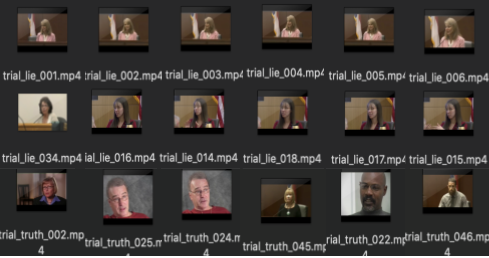
\includegraphics[width=12cm,keepaspectratio]{XX_Figures/Fig_DatasetTrial_Problem.png}
	\caption{\footnotesize  Algunos fotogramas de los videos del dataset utilizado en el modelo piloto.}
	\label{fig:Fig_DatasetTrial_Problem}
\end{figure}

Al analizar el conjunto de entrenamiento se observa que las clases están balanceadas (aproximadamente 50\% de datos de mentira 50\% de datos de verdad), pero existe el caso de que varios individuos aparecen en más videos a comparación con los demás. Este fenómeno se puede apreciar en la Figura \ref{fig:Fig_DatasetTrial_Problem} y puede tener como consecuencias que los parámetros de la red se estén ajustando a características particulares de los individuos que se repiten en más ocasiones y que no haya suficientes muestras para generalizar y evitar la memorización de los datos.\\

Una manera propuesta de probar esta hipótesis es utilizando las mismas arquitecturas probadas en `Trial' pero con otro conjunto de datos más equilibrado en videos, personas y tiempo. Si no existe un sobre ajuste en los modelos, entonces se puede concluir que el principal causante de sobreajuste en los modelos se debe al conjunto de datos limitado.\\

\begin{figure}[h!]
	\centering
	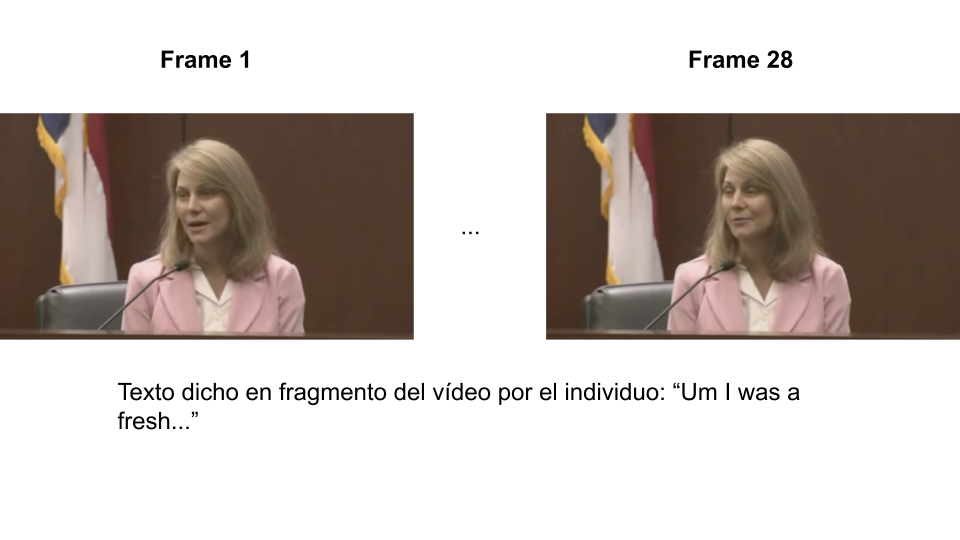
\includegraphics[width=14cm,keepaspectratio]{XX_Figures/TextoFragmento28Frames.png}
	\caption{\footnotesize Dato de 28 fotogramas con información irrelevante.}.
	\label{fig:TextoFragmento28Frames}
\end{figure}


Pese a que los modelos que tienen como entrada 28 fotogramas con FrameSpace = 1 (2s de información) contienen más información que el modelo piloto, aún no es suficiente tiempo para tener una declaración completa del individuo en varios de los datos y esto puede causar una problemática para clasificar correctamente los datos. Este fenómeno se observa en la Figura \ref{fig:TextoFragmento28Frames}.


\subsubsection{Problemáticas}
\label{sec:ProblematicasVariantesModeloPilotoTrial}

La problemática de estos modelos se listan en la tabla \ref{tab:ProblematicasVariantesMPiloto} con el Id \textbf{1B}.

\begin{table}[h!]
\centering
    \begin{tabular}{|p{1cm}|p{3cm}|p{3cm}|p{7cm}|}
        \hline 
        Id & Problemática & Posibles causas & Descripción\tabularnewline
        \hline 
        \hline 
        \multirow{3}{*}{1A} & \multirow{2}{*}{Overfitting} & Gran cantidad de parámetros & La arquitectura tiene los parámetros suficiente para memorizar los
        datos de entrenamiento.\tabularnewline
        \cline{2-4} \cline{3-4} \cline{4-4} 
         & Etiquetado Erróneo & Poca información  & 7 fotogramas (1/4s) es muy poca información para contener una mentira
        o una verdad.\tabularnewline
        \hline 
        \multirow{2}{*}{1B} & Overfitting & Conjunto de datos pequeño & Debido a que el dataset es pequeño o no tiene los suficientes ejemplos
        para generalizar, puede causar overfitting en los datos de entrenamiento.\tabularnewline
        \cline{2-4} \cline{3-4} \cline{4-4} 
         & Etiquetado Erróneo2 & Poca información  & 28 fotogramas con FrameSpace = 1 (2s) es muy poca información para contener
        una mentira o una verdad.\tabularnewline
        \hline 
    \end{tabular}
    \caption{\footnotesize  Problemáticas de las variantes del modelo piloto.}.
    \label{tab:ProblematicasVariantesMPiloto}
\end{table}
%---------------------------------
%---------------------------------
%---------------------------------
%---------------------------------
%---------------------------------
%---------------------------------

\subsection{Variantes del modelo piloto Dataset `Interview'}
\label{sec:VariantesModeloPilotoInterview}

En esta sección se probaron varias arquitecturas similares mostradas en la sección anterior con la diferencia de que el conjunto de datos es distinto y casi tres veces mayor que el anterior. Esto con el objetivo de probar la hipótesis planteada en la que se menciona que al tener un conjunto de datos limitado afecta el desempeño de la red causando sobreajuste y al obtener más cantidad de información para el entrenamiento evita el sobreajuste.

%\begin{figure}[p]
%    	\centering
%    	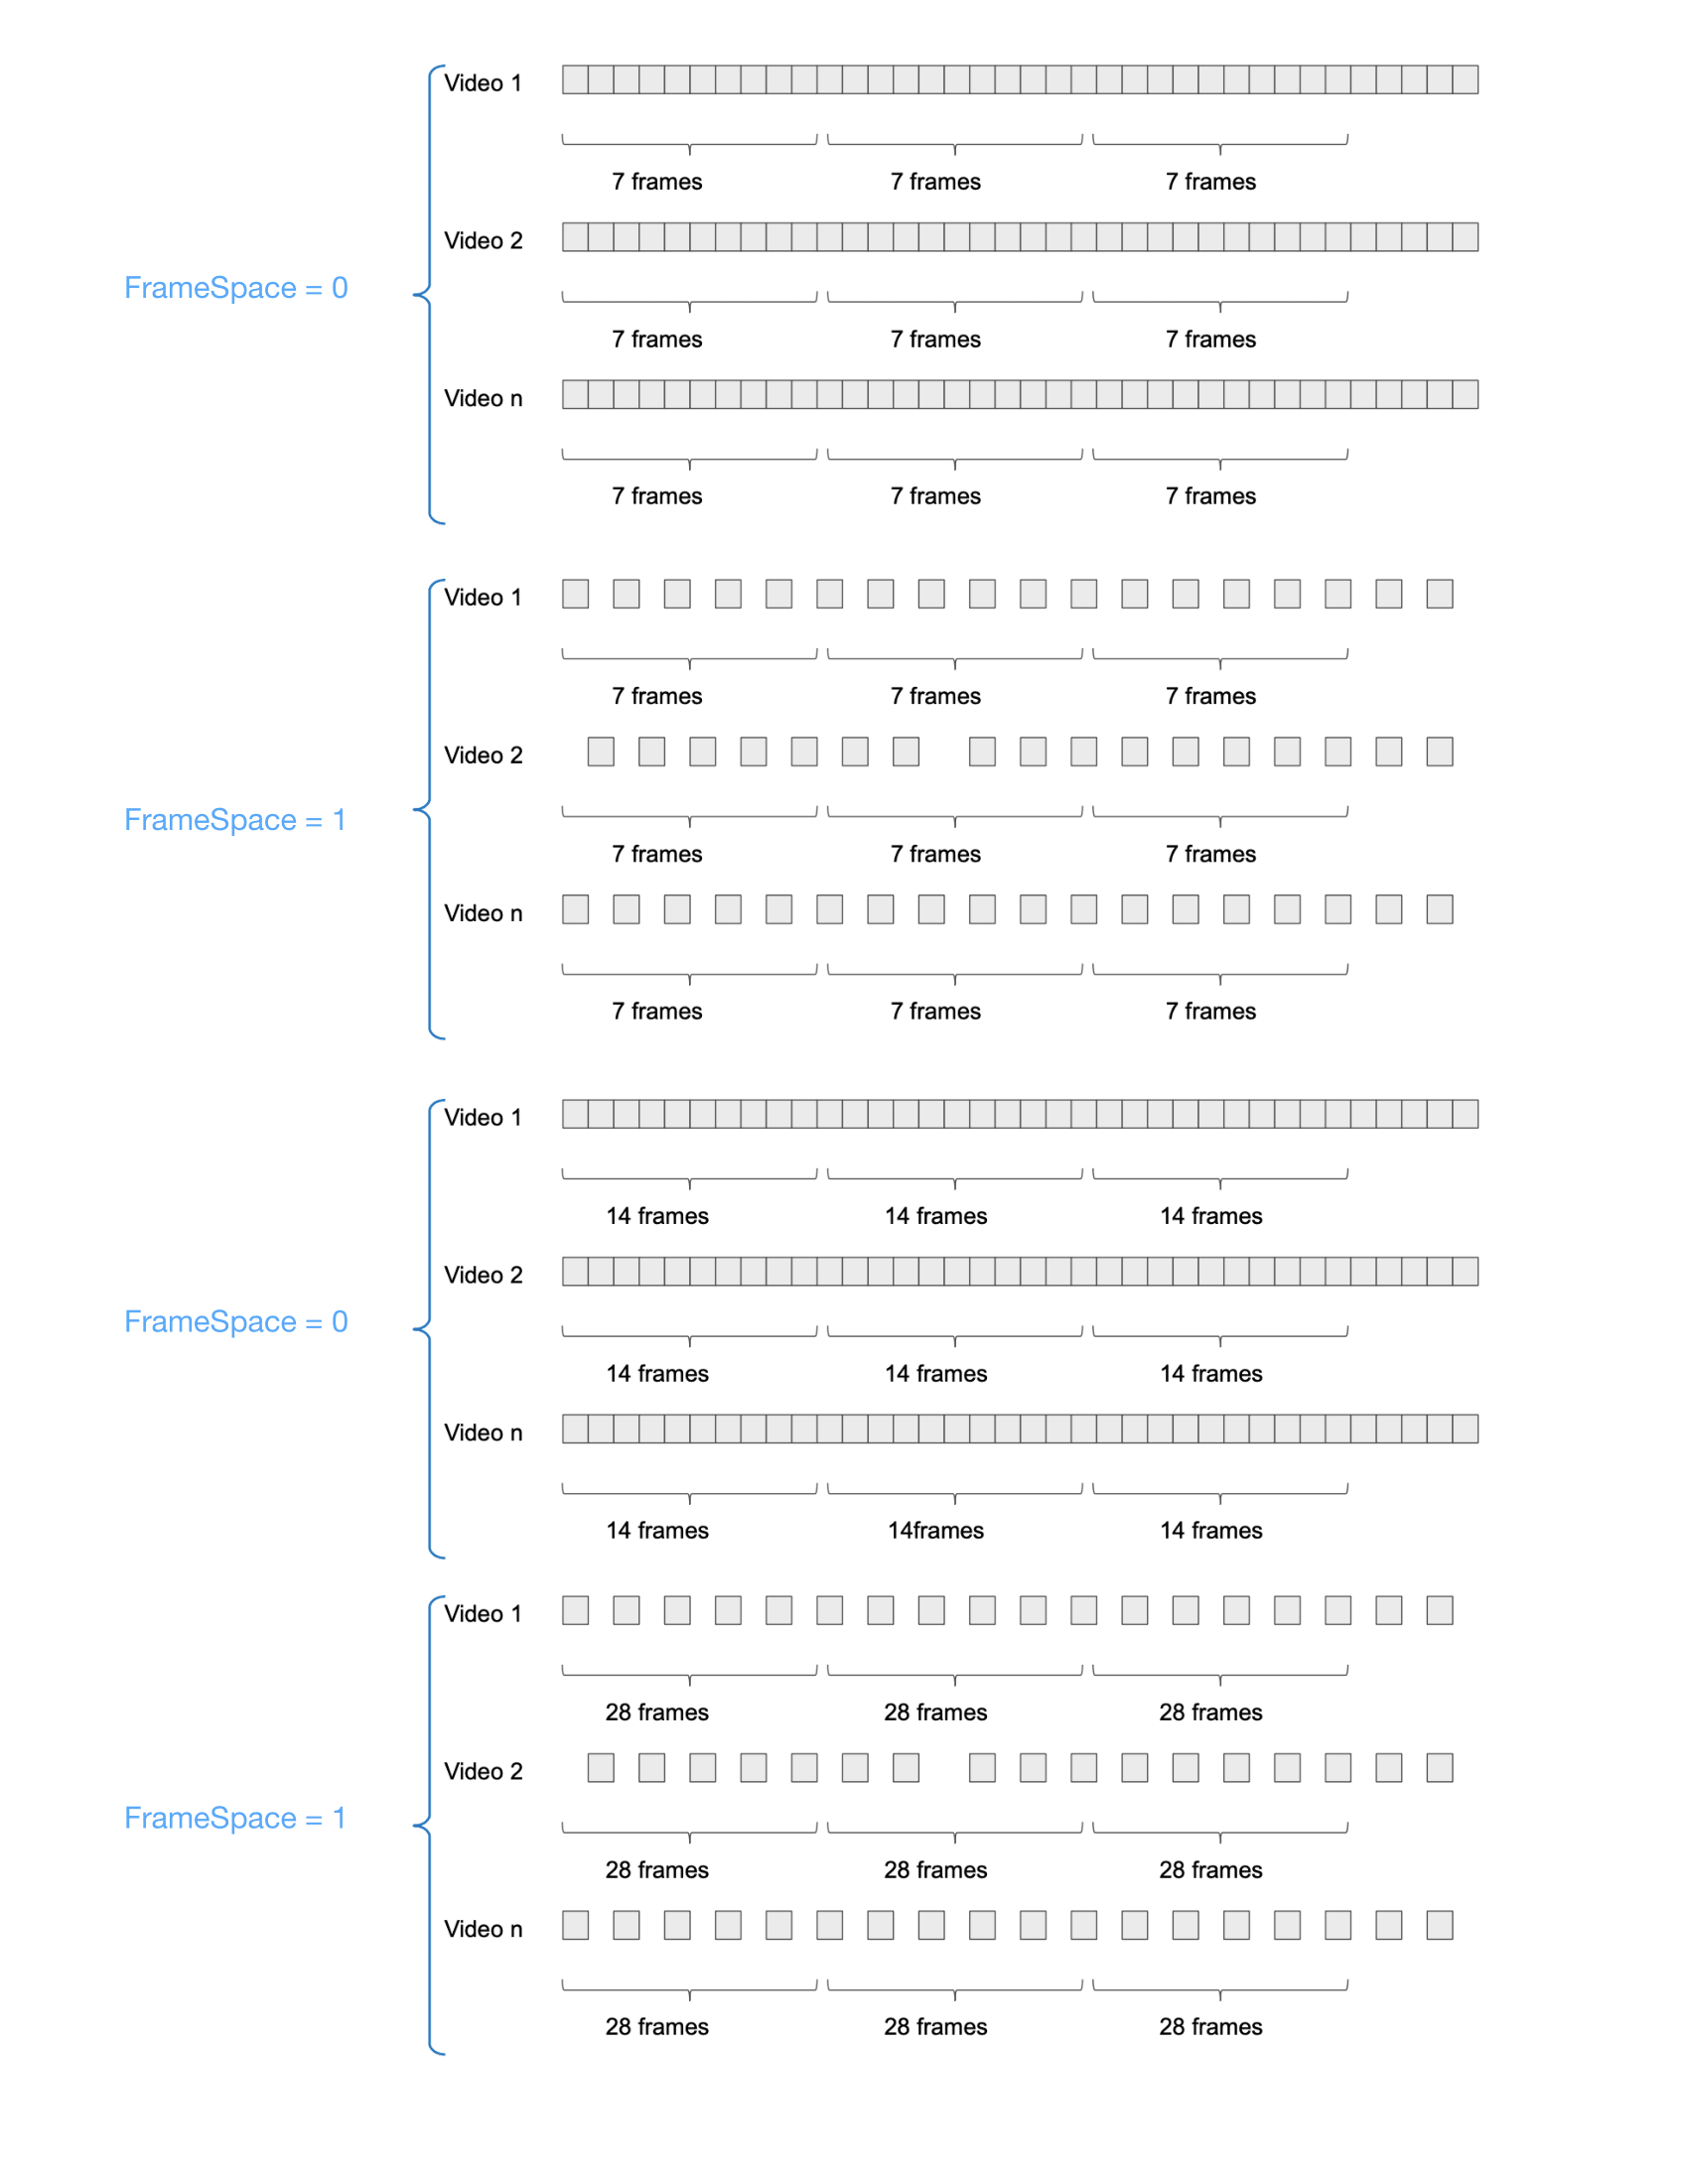
\includegraphics[width=18cm,keepaspectratio]{XX_Figures/Fig_Dataset1_7_14_28F.png%}
%    	\caption{\small División de los videos en datos de 7, 14 y 28 frames con %diferente FrameSpace.}
%    	\label{fig:Fig_Dataset1_7_14_28F}
%\end{figure}

%\subsubsection{Descripción del modelo}
%\label{sec:DescripcionVariantesModeloPilotoInterview}

%Modelo \textbf{3D-[2a]DS-[4]CH-[1]Fr-[2]FC-[14]MP-[50]DO}\\

%Modelo \textbf{3D-[2a]DS-[7]CH-[2]Fr-[5]FC-[4]MP-[50]DO}\\

%Modelo \textbf{3D-[2a]DS-[3]CH-[3]Fr-[11]FC-[15]MP-[50]DO}\\
%---------------------------------------------------
\subsubsection{Tabla de desempeño}
\label{sec:TDesempenoVariantesModeloPilotoInterview}

\begin{table}[h!]
\centering
        \begin{tabular}{|c|c|c|c|}
        \hline 
        Modelo & Train & Val & Test\tabularnewline
        \hline 
        \hline 
        3D-{[}2a{]}DS-{[}4{]}CH-{[}1{]}Fr-{[}2{]}FC-{[}14{]}MP-{[}0{]}DO-[2]LR-[4]BS & 52\% & 50\% & 50\%\tabularnewline
        \hline 
        3D-{[}2a{]}DS-{[}7{]}CH-{[}2{]}Fr-{[}5{]}FC-{[}4{]}MP-{[}0{]}DO-[2]LR-[3]BS & 53\% & 50\% & 50\%\tabularnewline
        \hline 
        3D-{[}2a{]}DS-{[}3{]}CH-{[}3{]}Fr-{[}11{]}FC-{[}15{]}MP-{[}0{]}DO-[2]LR-[2]BS & 57\% & 62\% & 50\%\tabularnewline
        \hline 
    \end{tabular}
    \caption{\footnotesize  Tres variantes del modelo piloto utilizando Dataset `Interview'.}.
    \label{tab:RVariantesPilotoInterview}
\end{table}

En la Tabla \ref{tab:RVariantesPilotoInterview} se observa que los modelos obtuvieron un accuracyData del 52\% al 57\% en el entrenamiento lo cuál muestra que no hay sobreajuste con este conjunto de datos más grande y equilibrado. Esto prueba que la hipótesis mencionada es correcta al decir que la poca cantidad de datos era la principal causa de sobreajuste en los modelos.\\

En estas pruebas los modelos no concluyeron el proceso de aprendizaje (underfitting) exitosamente a pesar de ser los mismos probados en la sección anterior. El ajuste bajo (underfitting) es el problema contrario al sobreajuste y es el caso donde el modelo no ha logrado aprender lo suficiente de los datos de entrenamiento lo que resulta en una generalización baja y predicciones poco confiables, al igual que el sobreajuste. Por lo general la razón más común del underfitting es la poca cantidad de parámetros en el modelo.\\

El ajuste bajo (underfitting) se puede combatir aumentando el número de características extraídas y las capas ocultas en la MLP pero debido a las entradas y a las operaciones  y limitaciones computacionales, no es posible aumentar el tamaño del modelo.

\begin{figure}[h!]
	\centering
	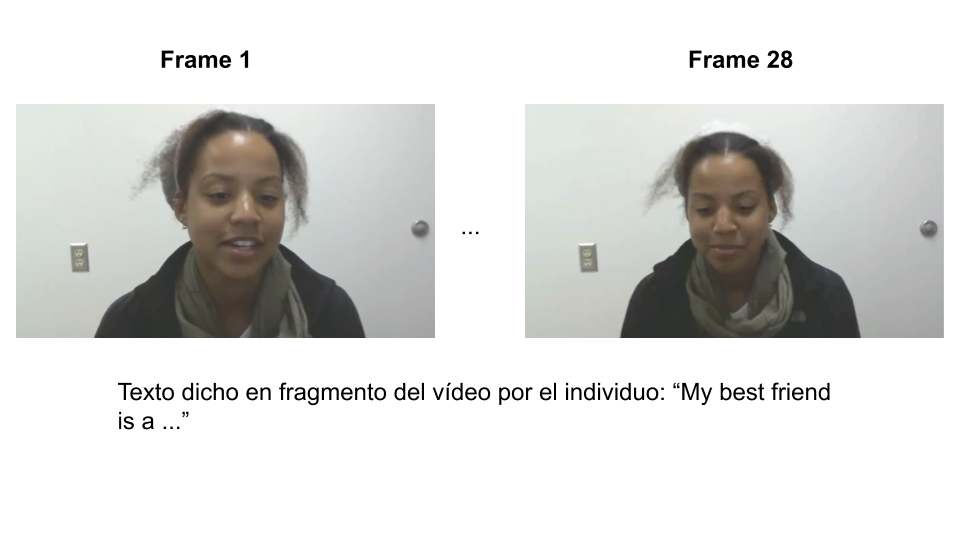
\includegraphics[width=14cm,keepaspectratio]{XX_Figures/TextoFragmento28FramesD2.png}
	\caption{\footnotesize Dato de 28 fotogramas con información irrelevante en el Dataset `Interview'.}.
	\label{fig:TextoFragmento28FramesD2}
\end{figure}

Los datos de 28 fotogramas con FrameSpace = 1 con el Dataset `Interview' tampoco tienen suficiente información para tener una declaración completa del individuo lo que puede causar problemáticas para clasificar correctamente los datos. Este fenómeno se observa en la Figura \ref{fig:TextoFragmento28FramesD2}.

\subsubsection{Problemáticas}
\label{sec:ProblematicasVariantesModeloPilotoTrial}

La problemática de este modelo se listan en la tabla \ref{tab:ProblematicasPilotointerview} con el Id \textbf{2C}.


\begin{table}[h!]
\centering
    \begin{tabular}{|p{1cm}|p{3cm}|p{3cm}|p{7cm}|}
        \hline 
        Id & Problemática & Posibles causas & Descripción\tabularnewline
        \hline 
        \hline 
        \multirow{3}{*}{1A} & \multirow{2}{*}{Overfitting} & Gran cantidad de parámetros & La arquitectura tiene los parámetros suficiente para memorizar los
        datos de entrenamiento.\tabularnewline
        \cline{2-4} \cline{3-4} \cline{4-4} 
         & Etiquetado Erróneo & Poca información  & 7 fotogramas (1/4s) es muy poca información para contener una mentira
        o una verdad.\tabularnewline
        \hline 
        \multirow{2}{*}{1B} & Overfitting & Conjunto de datos pequeño & Debido a que el dataset es pequeño o no tiene los suficientes ejemplos
        para generalizar, puede causar overfitting en los datos de entrenamiento.\tabularnewline
        \cline{2-4} \cline{3-4} \cline{4-4} 
         & Etiquetado Erróneo2 & Poca información  & 28 fotogramas con FrameSpace = 1 (2s) es muy poca información para contener
        una mentira o una verdad.\tabularnewline
        \hline 
        \multirow{3}{*}{2C} & Underfitting & Red Sencilla & Debido a las pocas caraterísticas extraídas o a la cantidad de capas
        ocultas en la MLP.\tabularnewline
        \cline{2-4} \cline{3-4} \cline{4-4} 
         & Etiquetado Erróneo & Poca información  & 28 fotogramas con FrameSpace = 1 (2s) es muy poca información para contener
        una mentira o una verdad.\tabularnewline
        \cline{2-4} \cline{3-4} \cline{4-4} 
         & PCcapacity & Operaciones Computacionales & El tener más cantidad de fotogramas requiere más operaciones computacionales
        por capas convolucionales y extraer más cantidad de características. La capacidad computacional con las operaciones propuestas es limitada.\tabularnewline
        \hline 
    \end{tabular}
    \caption{\footnotesize Problemáticas de las variantes del modelo piloto con el Dataset `Interview'.}.
    \label{tab:ProblematicasPilotointerview}
\end{table}

%---------------------------------
%---------------------------------
%---------------------------------
%---------------------------------


\section{ Modelo 3DLargeFramesMultiChannels}
\label{sec:3DDNN-100F-MultiChannels-FS-TS}

Este modelo tiene la finalidad de combatir la poca información de los fotogramas que existía en los otros modelos tomando datos con gran cantidad de información. La limitación de tener más neuronas para la extracción de características que ayuden a combatir el underfitting que se tuvo en la sección \ref{sec:VariantesModeloPilotoInterview}, se combatió al tener fotogramas más pequeños (0.25 veces más pequeño) y aumentando el TemporalStride a dos en las capas Maxpooling para reducir el número de capas y operaciones convolucionales 3D.


\subsection{Descripción del Modelo}
\label{sec:DescripcionModeloLarge}

Nomenclatura Modelo 3DLargeFramesMultiChannels: \textbf{3D-[2a]DS-[3]CH-[4]Fr-0[12]FC-[16]MP-[0]DO-[1]LR-[0]BS}\\

Según la nomenclatura propuesta, la arquitectura de red consiste:\\

\begin{itemize}
    \item {[2a]DS}
        \begin{itemize}
            \item Dataset utilizado `Interview'
            \item Imágenes de 50x50 en la que aparece el rostro, hombros y brazos de una persona.
    \end{itemize}
    
    \item {[3]CH}
        \begin{itemize}
            \item Canales GS, SX, SY
    \end{itemize}

    \item {[4]Fr}
        \begin{itemize}
            \item Datos de 100 fotogramas
            \item FrameSpace 2
            \item Frames per Convolution (9,7,7,7)
            \item TemporalStride (2,2,2,2)
    \end{itemize}
    
    \item {[12]FC}
        \begin{itemize}
            \item Features per Convolution (16,32,128,256)
    \end{itemize}
    
    \item {[16]MP}
        \begin{itemize}
            \item 768 neuronas en la capa de entrada de la MLP con función de activación ReLu, 128 neuronas en las 9 capas ocultas con función de activación ReLu y 2 neuronas en la capa de salida con función SoftMax.
    \end{itemize}
    
    \item {[0]DO}
        \begin{itemize}
            \item Dropout 0\%
    \end{itemize}
    
    \item {[1]LR}: indica que se está ocupando una tasa de aprendizaje de 0.001 para el optimizador Adam.
    
     \item {[0]BS}: indica que el tamaño del lote (batch size) es de 100 datos para el entrenamiento.

\end{itemize}

\subsection{Tabla de desempeño}
\label{sec:TablaDesempeno}

\begin{table}[th]
\centering
    \begin{tabular}{|c|c|c|c|}
        \hline 
        Modelo & Train & TestPO & TestWI\tabularnewline
        \hline 
        \hline 
        3D-{[}2a{]}DS-{[}3{]}CH-{[}4{]}Fr-0{[}12{]}FC-{[}16{]}MP-{[}0{]}DO-[1]LR-[0]BS & 93\% & 53\% & \textbf{63}\%\tabularnewline
        \hline 
    \end{tabular}
    \caption{Accuracy obtenido por el modelo 3DLargeFramesMultiChannels}.
    \label{tab:TDesempeno3DLargeFramesMultiChannels}
\end{table}

Se observa en la Tabla \ref{tab:TDesempeno3DLargeFramesMultiChannels} que se soluciona el problema de underfitting que tenía el anterior modelo. Se tuvo que eliminar la regularización por Dropout ya que el modelo no lograba entrenar. También fue necesario extraer más características en la red 3D Convolucional y aumentar el número de capas ocultas en la MLP con el costo de que con el paso de las épocas de entrenamiento el modelo tiende a sobre ajustarse. También se observa que el modelo tuvo mejor desempeño en las pruebas de las personas que ya conocía (TestWI) obteniendo un 63\% de accuracyData pero un 53\% de accuracyData en las pruebas de las personas que desconocía (TestPO). Una hipótesis que explica este fenómeno, es que el modelo ha logrado extraer características que particularmente delatan mentira en individuos con los que previamente fue entrenado pero no es capaz de generalizar las características que delatan mentira en todas las personas, dando como resultado un mejor accuracyData en las pruebas con personas conocidas y peor accuracy con personas desconocidas. Bashar \cite{Rajoub2014ThermalDetection} menciona que existen varios trabajos que obtuvieron resultados similares en la que sus modelos tenían pésimos resultados en las pruebas con personas distintas a los datos de entrenamiento (Train) y mejores resultados con personas que también se encuentran en los datos de entrenamiento. \\

Una desventaja de extraer características en videos por medio de redes convolucionales 3D es que todos los datos de entrada deben de coincidir con la misma dimensión espacial, dimensión de canales y dimensión temporal. Esto limita al modelo a tener como entrada, datos con diferente duración de tiempo y en pruebas reales la mayor parte de los videos tienen diferente duración. A pesar de que el Dataset 'Interview' contiene datos balanceados, la duración de los videos no es la misma.\\

\begin{figure}[h!]
	\centering
	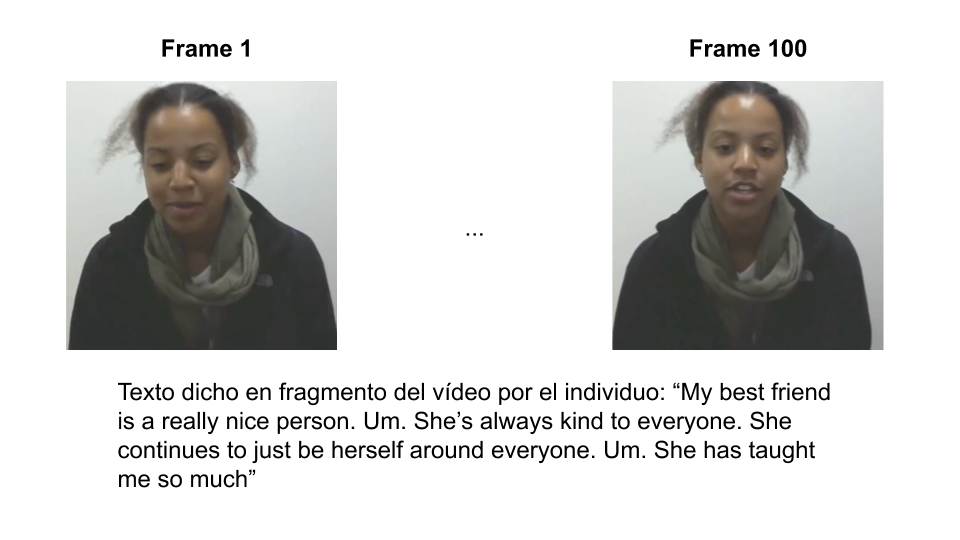
\includegraphics[width=14cm,keepaspectratio]{XX_Figures/TextoFragmento100FramesD2.png}
	\caption{\footnotesize Dato de 100 fotogramas con varias declaraciones de verdad en el Dataset `Interview'.}.
	\label{fig:TextoFragmento100FramesD2}
\end{figure}

\begin{table}[p!]
\centering
    \begin{tabular}{|p{1cm}|p{3cm}|p{3cm}|p{7cm}|}
        \hline 
        Id & Problemática & Posibles causas & Descripción\tabularnewline
        \hline 
        \hline 
        \multirow{3}{*}{1A} & \multirow{2}{*}{Overfitting} & Gran cantidad de parámetros & La arquitectura tiene los parámetros suficiente para memorizar los
        datos de entrenamiento.\tabularnewline
        \cline{2-4} \cline{3-4} \cline{4-4} 
         & Etiquetado Erróneo & Poca información  & 7 fotogramas (1/4s) es muy poca información para contener una mentira
        o una verdad.\tabularnewline
        \hline 
        \multirow{2}{*}{1B} & Overfitting & Conjunto de datos pequeño & Debido a que el dataset es pequeño o no tiene los suficientes ejemplos
        para generalizar, puede causar overfitting en los datos de entrenamiento.\tabularnewline
        \cline{2-4} \cline{3-4} \cline{4-4} 
         & Etiquetado Erróneo2 & Poca información  & 28 fotogramas con FrameSpace = 1 (2s) es muy poca información para contener
        una mentira o una verdad.\tabularnewline
        \hline 
        \multirow{3}{*}{2C} & Underfitting & Red Sencilla & Debido a las pocas caraterísticas extraídas o a la cantidad de capas
        ocultas en la MLP.\tabularnewline
        \cline{2-4} \cline{3-4} \cline{4-4} 
         & Etiquetado Erróneo2 & Poca información  & 28 fotogramas con FrameSpace = 1 (2s) es muy poca información para contener
        una mentira o una verdad.\tabularnewline
        \cline{2-4} \cline{3-4} \cline{4-4} 
         & PCcapacity & Operaciones Computacionales & El tener más cantidad de fotogramas requiere más operaciones computacionales
        por capas convolucionales y extraer más cantidad de características.
        La capacidad computacional con las operaciones propuestas est limitada.\tabularnewline
        \hline 
        \multirow{2}{*}{2D} & \multirow{2}{*}{Overfitting} & Gran cantidad de parámetros & Debido a que es necesario tener una red lo suficientemente grande
        para combatir el underfitting, el modelo ahora tiende al overfitting
        con el paso de las épocas.\tabularnewline
        \cline{3-4} \cline{4-4} 
         &  & No Dropout & Tener un Dropout fijo evita que la red logre terminar el proceso de
        entrenamiento pero al no tener Dropout ayuda a que la red se sobre
        ajuste a los datos de entrenamiento.\tabularnewline
        \hline 
    \end{tabular}
    \caption{Problemáticas actuales de los modelos propuestos.}.
    \label{tab:TablaProblematicas3DLargeFramesMultiChannels}
\end{table}

Al tener datos de 100 fotogramas con FrameSpace = 2 se tiene aproximadamente 10s de información y con esto es suficiente para al menos tener una declaración completa de mentira o verdad, como se muestra en la Figura \ref{fig:TextoFragmento100FramesD2}, solucionando el problema con el etiquetado erróneo mostrados en la sección \ref{sec:Modelos_pilotos}.\\

Si se propone un modelo con redes convolucionales 3D que tengan datos con más cantidad de fotogramas, puede causar la perdida de muchos datos que no cumplan con la cantidad mínima de fotogramas. El 100\% de los datos en el Dataset `Interview' contienen al menos un dato con 10s de información , evitando la perdida de videos y de individuos en el entrenamiento y en las pruebas.\\

La métrica utilizada (Ecuación \ref{equ:Accuracy}) evalúa cuántos datos de 100 fotogramas fueron etiquetados correctamente pero no nos muestra cuántos videos fueron etiquetados correctamente, dando como consecuencia que este modelo en pruebas reales no de suficiente información para decidir si un video es clasificado como mentira o verdad.



\subsection{Problemáticas}
\label{sec:Problematicas3DLargeFramesMultiChannels}

La problemática de este modelo se listan en la tabla \ref{tab:TablaProblematicas3DLargeFramesMultiChannels} con el Id \textbf{2D}.


%------------------------
%------------------------
%------------------------

\section{ Modelo 3DLargeFramesMultiChannelsDV}
\label{sec:3DLargeFramesMultiChannelsDV}

Este modelo tiene la finalidad de combatir el sobreajuste. Para esto se propone un algoritmo de Dropout Variable en el cuál consiste en aumentar la probabilidad de desconexión de las neuronas cuando el modelo comienza a obtener un accuracyData mayor al 60 \% en el conjunto de entrenamiento.\\

También se propone utilizar una la métrica para evaluar si un video pertenece a la clase mentira o a la clase verdad. A través de la métrica AccuracyPerVideos se logra esto y en la Figura \ref{fig:Fig_AccuracyPerVideoEjemplo} se muestra un ejemplo de cómo se decide si un video pertenece a una clase de verdad o una clase de mentira. El primer video tiene 3 datos de 100f, cada uno con etiqueta de verdad; Al momento de evaluar el sistema se obtienen 2 datos clasificados como verdad y uno como mentira, dando una probabilidad del 66.6\%  de pertenecer a la case verdad y como coincide con la etiqueta global del video, entonces es un video clasificado correctamente.\\

El algoritmo de Dropout Variable (DV) es el siguiente:\\

\begin{algorithm}[h!]
\SetAlgoLined
\KwResult{Dropout}
 \textbf{ValorDeCastigo} = 40\\
 \textbf{AccuracyMinimo} = 60\\
 \eIf{$AccuracyTraining \geq AccuracyMinimo$}{
   Dropout = AccuracyTraining - ValorDeCastigo\;
   }{
   Dropout = 0\;
  }
 \caption{Algoritmo de Dropout Variable}
 \label{alg:DV}
\end{algorithm}

\begin{figure}[th]
	\centering
	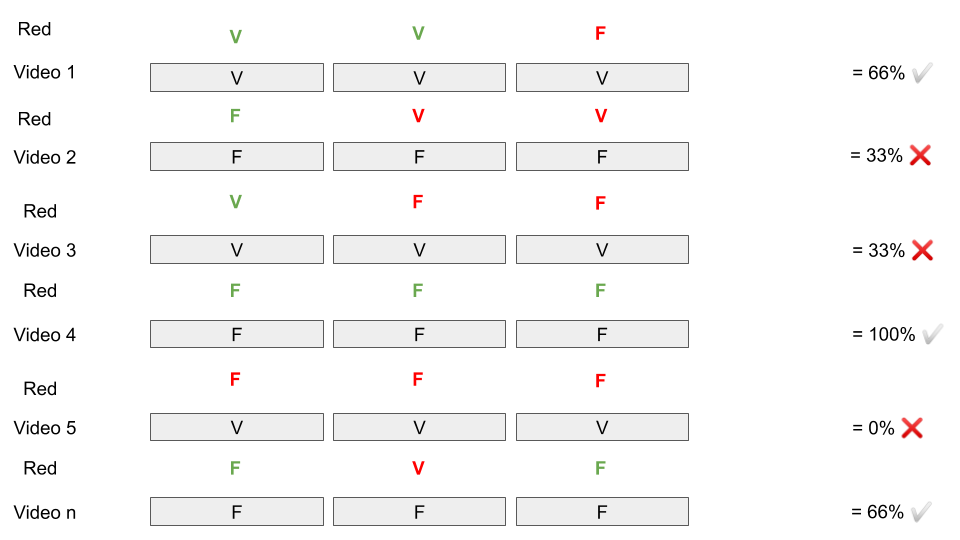
\includegraphics[width=16cm,keepaspectratio]{XX_Figures/Fig_AccuracyPerVideoEjemplo.png}
	\caption{\footnotesize Ejemplo de la aplicación de AccuracyPerVideo.}
	\label{fig:Fig_AccuracyPerVideoEjemplo}
\end{figure}

\subsection{Descripción del Modelo}
\label{sec:Descripcion3DLargeFramesMultiChannelsDV}

Nomenclatura Modelo 3DLargeFramesMultiChannelsDV: \textbf{3D-[2b]DS-[3]CH-[4]Fr-[13]FC-[17]MP-[DV]DO-[2]LR-[1]BS}\\

Según la nomenclatura propuesta, la arquitectura de red consiste:\\

\begin{itemize}
    \item {[2b]DS}
        \begin{itemize}
            \item Dataset utilizado `Interview'
            \item Imágenes de 50x50 en la que aparece el rostro de una persona.
    \end{itemize}
    
    \item {[3]CH}
        \begin{itemize}
            \item Canales GS, SX, SY
    \end{itemize}

    \item {[4]Fr}
        \begin{itemize}
            \item Datos de 100 fotogramas
            \item FrameSpace 2
            \item Frames per Convolution (9,7,7,7)
            \item TemporalStride (2,2,2,2)
    \end{itemize}
    
    \item {[12]FC}
        \begin{itemize}
            \item Features per Convolution (4,8,16,32)
    \end{itemize}
    
    \item {[16]MP}
        \begin{itemize}
            \item 96 neuronas en la capa de entrada de la MLP con función de activación ReLu, 1024 neuronas en las 9 capas ocultas con función de activación ReLu y 2 neuronas en la capa de salida con función SoftMax.
    \end{itemize}
    
    \item {[DV]DO}: Dropout variable
    
    \item {[2]LR}: indica que se está ocupando una tasa de aprendizaje de 0.001 para el optimizador Adam.
    
     \item {[1]BS}: indica que el tamaño del lote (batch size) es de 150 datos para el entrenamiento.
\end{itemize}



\subsection{Tabla de desempeño}
\label{sec:TDesempeno3DLargeFramesMultiChannelsDV}

En esta tabla se añadieron 2 AccuracyPerVideo. TestPO\_Vid da el porcentaje de videos que fueron clasificados correctamente con las pruebas TestPO y TestPO\_Vid indica el porcentaje de videos que fueron clasificados correctamente con las pruebas TestWI.
\begin{table}[h!]
\centering
    \begin{tabular}{|c|c|c|c|c|c|}
        \hline 
        Modelo & Train & TestPO & TestWI & TestPO\_Vid & TestWI\_Vid\tabularnewline
        \hline 
        \hline 
        3DLargeFramesMultiChannelsDV & 82\% & 53\% & \textbf{67\% } & 47\%  & \textbf{82\% }\tabularnewline
        \hline 
    \end{tabular}
    \caption{Desempeño del modelo 3DLargeFramesMultiChannelsDV.}.
    \label{tab:TablaProblematicas3DLargeFramesMultiChannelsDV}
\end{table}

Se obtuvo un mejor desempeño en las pruebas con el conjunto TestWI y el mismo desempeño que con el anterior modelo en el conjunto TestPO. Esto indica que el modelo propuesto es capaz de extraer características que ayuden a clasificar si una persona miente o dice una verdad, pero estas características pueden ser muy particulares de los individuos con los que fue entrenado; por esta razón al momento de evaluar las pruebas con los mismos individuos pero diferentes declaraciones, la red obtiene mejores resultados que cuando la red desconoce a los individuos de prueba. 
Esto puede indicar que la red deba ser calibrada (entrenar con las personas de prueba) para dar un mejor desempeño en las pruebas.\\

\begin{figure}[th]
	\centering
	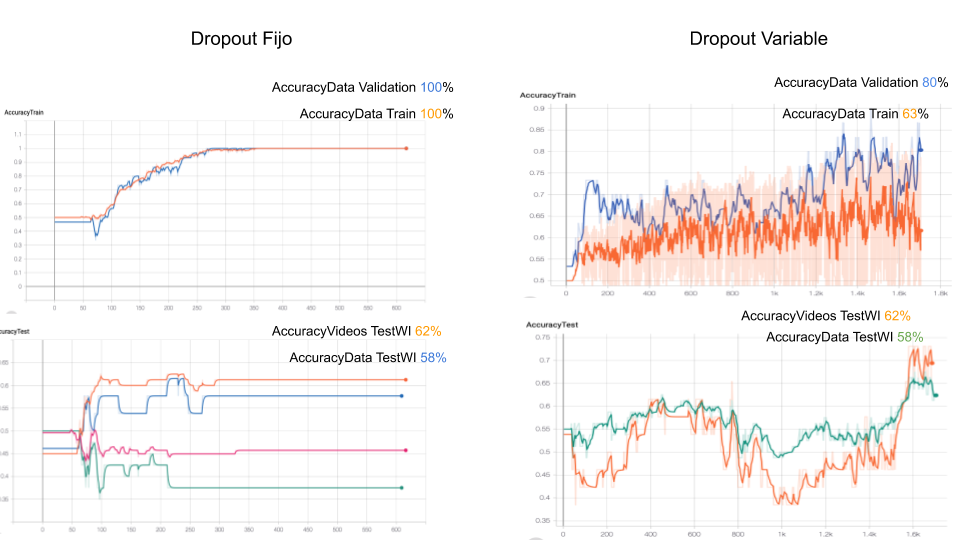
\includegraphics[width=18cm,keepaspectratio]{XX_Figures/DropoutVariable.png}
	\caption{\footnotesize Modelo con dropout fijo a la izquierda y dropout variable a la derecha.}
	\label{fig:DropoutVariable}
\end{figure}

En la Figura \ref{fig:DropoutVariable}, se observan dos modelos con los mismos hiperparámetros, el de la izquierda no contiene dropout y el de la derecha contiene dropout variable; el modelo sin dropout a pesar de tener un incremento del accuracy casi continuo con el paso de las épocas, tendía al sobreajuste que causó un estancamiento en el AccuracyPerVideo TestWI y AccuracyPerData TestWI a partir de la época 300 en adelante. En cambio en las pruebas con dropout variable se muestra que a pesar de tener un proceso de aprendizaje más forzado, las pruebas TestWI van teniendo un mejor desempeño en las últimas épocas.\\

Este ejemplo muestra que los modelos con dropout variable tienden a tener mejores resultados en las pruebas (específicamente con TestWI) con el paso de las épocas que los modelos con dropout fijo.\\

\subsection{Problemáticas}
\label{sec:Problematicas3DLargeFramesMultiChannelsDV}

La problemática de este modelo es el desempeño con nuevos individuos. Las posibles razones se en listan en la tabla \ref{tab:TablaProblematicas3DLargeFramesMultiChannelsDV} con el Id \textbf{2E}.\\


\begin{table}[h!]
\centering
    \begin{tabular}{|p{1cm}|p{3cm}|p{3cm}|p{7cm}|}
    \hline 
    Id & Problemática & Posibles causas & Descripción\tabularnewline
    \hline 
    \hline 
    \multirow{3}{*}{1A} & \multirow{2}{*}{Overfitting} & Gran cantidad de parámetros & La arquitectura tiene los parámetros suficiente para memorizar los
    datos de entrenamiento.\tabularnewline
    \cline{2-4} \cline{3-4} \cline{4-4} 
     & Etiquetado Erróneo & Poca información & 7 fotogramas (1/4s) es muy poca información para contener una mentira
    o una verdad.\tabularnewline
    \hline 
    \multirow{2}{*}{1B} & Overfitting & Conjunto de datos pequeño & Debido a que el dataset es pequeño o no tiene los suficientes ejemplos
    para generalizar, puede causar overfitting en los datos de entrenamiento.\tabularnewline
    \cline{2-4} \cline{3-4} \cline{4-4} 
     & Etiquetado Erróneo2 & Poca información & 28 fotogramas con FrameSpace = 1 (2s) es muy poca información para contener
    una mentira o una verdad.\tabularnewline
    \hline 
    \multirow{3}{*}{2C} & Underfitting & Red Sencilla & Debido a las pocas caraterísticas extraídas o a la cantidad de capas
    ocultas en la MLP.\tabularnewline
    \cline{2-4} \cline{3-4} \cline{4-4} 
     & Etiquetado Erróneo2 & Poca información & 28 fotogramas con FrameSpace = 1 (2s) es muy poca información para contener
    una mentira o una verdad.\tabularnewline
    \cline{2-4} \cline{3-4} \cline{4-4} 
     & PCcapacity & Operaciones Computacionales & El tener más cantidad de fotogramas requiere más operaciones computacionales
    por capas convolucionales y extraer más cantidad de características.
    La capacidad computacional con las operaciones propuestas est limitada.\tabularnewline
    \hline 
    \multirow{2}{*}{2D} & \multirow{2}{*}{Overfitting} & Gran cantidad de parámetros & Debido a que es necesario tener una red lo suficientemente grande
    para combatir el underfitting, el modelo ahora tiende al sobreajuste
    con el paso de las épocas.\tabularnewline
    \cline{3-4} \cline{4-4} 
     &  & No Dropout & Tener un dropout fijo evita que la red logre terminar el proceso de
    entrenamiento pero al no tener Dropout ayuda a que la red se sobre
    ajuste a los datos de entrenamiento.\tabularnewline
    \hline 
    2E & No Generalization & Calibración & Debido a que el modelo tiene mejores resultados en las pruebas con
    personas conocidas y malos resultados con personas desconocidas. Por
    lo tanto este modelo entrenado con el conjunto de datos `Interview' no es capaz
    de generalizar el problema de detección de mentiras\tabularnewline
    \hline 
    \end{tabular}

    \caption{Problemática del modelo 3DLargeFramesMultiChannelsDV}.
    \label{tab:TablaProblematicas3DLargeFramesMultiChannelsDV}
\end{table}


En la tabla \ref{tab:ComparandoModelo}, se observa el modelo propuesto junto con algunos trabajos del estado del arte y las diferentes metodologías que se utilizan para detectar mentiras. Con \textbf{Extracción de Características Manuales} se refiere a que los modelos propuestos requieren de algún humano que haya etiquetado características extraídas manualmente, como el etiquetado de la microexpresión en algún punto del video, etiquetado de cuántas veces la persona evadió la mirada, entre otros. \textbf{Texto} se refiero a que los modelos requirieron de procesar texto, con \textbf{Audio} requieren de procesar la señal de audio del video, \textbf{LNV} se refiere a que se necesita de video para diferentes análisis del Lenguaje no verbal, \textbf{Fisiológico} indica que se necesita extraer valores de reacciones fisiológicas e \textbf{Instrumentos Especializados} menciona si se requirió de instrumentación especializada para realizar los experimentos. Con los resultados obtenidos de nuestro modelo propuesto y los del estado del arte se muestra que se obtiene un buen porcentaje para clasificar mentiras y verdades en videos  específicamente con las pruebas Test-Within (TestWI), pero un mal porcentaje para clasificar mentiras en las pruebas Test-Leave-one-person-out (TestPO), mostrando que el modelo no es capaz de generalizar la clasificación para todos los individuos pero si para los individuos con los que fue previamente entrenado el modelo.

\begin{table}[h!]
\centering
\begin{turn}{90}
    \begin{tabular}{|p{4cm}|p{3cm}|c|c|c|c|p{3 cm}|c|c|}
        \hline 
        Modelo & Extracción de características manuales & Texto & Audio & LNV & Fisiológico & Instrumentos Especializados & TestPO & TESTWI\tabularnewline
        \hline 
        \hline 
        Warmeling et al. 2011 & - & - & - & \checkmark & \checkmark & \checkmark & - & 66\%\tabularnewline
        \hline 
        Verónica et al. 2015 & \checkmark & \checkmark & \checkmark & \checkmark & - & - & - & 75\%\tabularnewline
        \hline 
        Donald Grubin (Polygraph study) et al. 2005 & \checkmark & - & - & - & \checkmark & \checkmark & - & 81\%\tabularnewline
        \hline 
        \cellcolor{lightgray}\textbf{3DLargeFrames MultiChannelsDV} & \cellcolor{lightgray}- & \cellcolor{lightgray}- & \cellcolor{lightgray}- & \cellcolor{lightgray}\checkmark & \cellcolor{lightgray}- & \cellcolor{lightgray}- & \cellcolor{lightgray}47\% & \cellcolor{lightgray}82\%\tabularnewline
        \hline 
        Verónica et al. 2016 & \checkmark & \checkmark & \checkmark & \checkmark & - & - & 58\% & 82\%\tabularnewline
        \hline 
        Bashar et al. 2014 & \checkmark & - & - & \checkmark & \checkmark & \checkmark & 58\% & 87\%\tabularnewline
        \hline 
        Abouelenien et al. 2016 & \checkmark & - & - & \checkmark & \checkmark & \checkmark & 61\% & -\tabularnewline
        \hline 
        Tsiamyrtzis et al. 2005 & \checkmark & - & - & \checkmark & \checkmark & \checkmark & 87\% & -\tabularnewline
        \hline 
        Krishnamurthy et al. 2018 & \checkmark & \checkmark & \checkmark & \checkmark & - & - & 96\% & -\tabularnewline
        \hline 
    \end{tabular}
    \end{turn}{90}
    \caption{Comparativa del modelo con estado del arte.}.
    \label{tab:ComparandoModelo}
\end{table}


\end{onehalfspacing}